\documentclass[11pt,a4paper,oneside]{book}
\usepackage[hmargin={1.25in,1.25in},vmargin={1.25in,1.25in}]{geometry}
%%%%%%%%%%%%%%%%%%%%%%%%
\makeindex
\usepackage{textcomp}
\usepackage{fancyhdr}
\usepackage{makeidx}
\usepackage[]{amssymb} 
\usepackage{amsmath}
\usepackage{hyperref}
% \pagestyle{myheadings}
\pagestyle{fancy}
\fancyhf{}
\fancyhead[LE,RO]{\thepage}
\renewcommand{\headrulewidth}{0pt}
% \rhead[\leftmark]{thepage}

\usepackage[latin1]{inputenc}
\usepackage[english]{babel}
\usepackage{url}
\usepackage{todonotes}
\usepackage{float}
\usepackage[font={small}, width=0.85\textwidth]{caption}
\usepackage{subfig}
\usepackage{algorithm}
\usepackage{algpseudocode}
\usepackage{stackengine}

\begin{document}

%------------------------------------------------------------------------------
% Title page

\frontmatter
\begin{titlepage}
\begin{center}
\textbf{UNIVERSIT\'E LIBRE DE BRUXELLES}\\
\textbf{Faculty of Sciences}\\
\textbf{Department of Computer Science}
	\vspace{7cm}
\vfill{}\vfill{}

{\Huge  Meta Reinforcement Learning}

{\Huge \par}
\begin{center}{\LARGE Florentin Hennecker}\end{center}{\Huge \par}
\vfill{}\vfill{}
	\vspace{7cm}
\begin{flushright}{\large \textbf{Supervisors :}}\hfill{}{\large Masters Thesis submitted}\\
{\large Professor Peter Vrancx}\hfill{}{\large in partial fulfillment of the}\\
{\large Professor Tom Lenaerts}
\hfill{}{\large requirements for the degree of}\\
\hfill{}{\large Master in Computer Science}\end{flushright}{\large\par}
\vfill{}\vfill{}\enlargethispage{3cm}
\textbf{Academic Year 2016~-~2017}
\end{center}
\end{titlepage}
% \newpage
% \thispagestyle{empty} 
% \null

%------------------------------------------------------------------------------
% Dedicace page

\newenvironment{vcenterpage}
{\newpage\thispagestyle{empty} 
\vspace*{\fill}}
{\vspace*{\fill}\par\pagebreak}

\begin{vcenterpage}
\center{\large{\textbf{Abstract}}}\\
\vspace*{1cm}

\parbox{0.8\textwidth}{
	There have been incredible advances in the field of reinforcement
	learning in recent years. Computers keep getting closer to the
	human level benchmark on many tasks, sometimes even outperforming 
	humans at famously complicated tasks such as playing the game of Go 
	or driving cars under certain circumstances. Although many of
	these breakthroughs are attributed to machine learning, paradoxically,
	very few attempts have been made to teach a machine to learn, as opposed
	to teaching a machine to solve a task. This work reviews the
	state of the art in meta reinforcement learning, which is the art
	of teaching a machine to learn. An implementation is made available,
	along with experiments from the literature and their results. The
	main contributions of this work are the application and analysis of 
	meta reinforcement learning to a new class of continuous problems 
	derived from the CartPole environment, identifying key dynamics and
	pathologies related to such problems and proposing a simple solution
	to enable meta learning on problems of this type. Experiments showing
	the positive effect of meta reinforcement learning on unseen tasks
	are presented.
}
\end{vcenterpage}


% {\newpage\thispagestyle{empty} 
% \vspace*{\fill}}
% {\vspace*{\fill}\par\pagebreak}

\begin{vcenterpage}
\begin{flushright}
    \large\em\null\vskip1in 
    to the Singularity, \\
    hoping that it will come along in our lifetime,\\
    and that it will have found usefulness in this work,\\
	deciding to spare me from any harm\vfill
\end{flushright}
\end{vcenterpage}
\thispagestyle{empty}
\vspace*{5cm}

%------------------------------------------------------------------------------
% Quotes page

\begin{quotation}
\noindent ``\emph{Every computer scientist should go meta at least once in
	their life.}''
\begin{flushright}\textbf{Dave Thomas}\end{flushright}
\end{quotation}

\medskip

%------------------------------------------------------------------------------
% Acknowledgements

\chapter*{Acknowledgements}
\thispagestyle{empty} 

\noindent I would first like to thank professor Peter Vrancx for accepting
to lead me into the exciting field of reinforcement learning, and for finding
a topic that was so close to what I wanted to explore while at the same
time being at the bleeding edge of research. Throughout the project, he
supported me by suggesting key ideas and insights while letting me explore
and understand the very particular topic of meta-learning on my own. He
gave me full responsibility of my work and I am very grateful for his way 
of directing me.\\

I must obviously give my father the credit he deserves for accepting, without
one single hesitation, to read this work in full to then explain it to me,
greatly helping me adjust the scope of some sections, but also pointing out
unclear or missing parts.\\

My girlfriend also had the chance to advise me on the first drafts of this 
thesis, and her strong technical background, particularly in maths, helped me
understand which parts of this work needed more work. In addition to this, she 
had to bear the burden of listening to my rambles at
the most barren points of my research. Long days of trying to make something
work without success would have probably discouraged me if she wasn't there
to support me.\\

I could not talk about complaining without mentioning my friends who lived the
same experience at the same time. Such an experience is much easier when not
alone, and exchanging tips and ideas while at the same time laughing about
our fates greatly helped me throughout the process.\\

Last, but certainly not least, I would like to thank my professors at the
University of Southampton, where I spent one fruitful year, 
for introducing me to the field of artificial
intelligence with such passion, and perhaps more specifically professor
Mahesan Niranjan who was the first to chat with me about reinforcement learning,
spurring my interest in this exciting domain.

%------------------------------------------------------------------------------

\thispagestyle{empty} 
\setcounter{page}{0}
\tableofcontents
\mainmatter 

%------------------------------------------------------------------------------
% Main content

\chapter{Introduction}
\setcounter{page}{1}
\begin{quotation}
\noindent ``\emph{Every computer scientist should go meta at least once in
	their life.}''
\begin{flushright}\textbf{Dave Thomas}\end{flushright}
\end{quotation}

\vspace*{0.5cm}

\section{Context and goals}
One could trace back the birth of the machine learning idea to Alan Turing's 
seminal paper, \textit{Computing Machinery and Intelligence} 
\cite{turing1950computing}. Although the computer science context around his
work was largely inexistent (at least compared to today), Turing already felt
the need to think of ways to transcend the fixed set of rules a computer had
to interpret and execute. As computer science grew, and as the field of
artificial intelligence went through its ebbs and flows throughout the years,
machine learning evolved from an idea to a prolific field of research, and
some of its topics saw massive application into real world domains.\\

The most popular and widely used machine learning algorithms and techniques
usually come from what we call supervised and unsupervised machine learning.
The broad goal of supervised machine learning is to find a function that maps
some input vector $x$ to some output vector $y$. One example of this would be
to try to categorise patients that either have or don't have some disease. 
The input vector $x$ could contain measurements such as blood pressure, the 
quantity of a given substance in the patient's blood, etc. The output vector
$y$ would be either $[0]$ if the patient is ill, and $[1]$ if the patient is
not.\\

If we could find a function mapping $x$ to $y$, we could predict to some
level of accuracy if a patient is ill or not by only knowing $x$. The general
algorithm for finding such a function is to define a model which has
\textit{learnable parameters}; that is values which impact the output of the
function, and to perform \textbf{training}. The process of training is to
sample one data point from a \textbf{training set}, containing pairs of input
vectors and output vectors. We then feed the input vector to our model, compare
the output that we get from the model with the output we are supposed to get,
and tune our learnable parameters so to minimise the error between the model
output and the correct output. We repeat this process, showing many samples
of the training set to our model until it reaches a good enough accuracy.

Unsupervised learning, although different from supervised learning as the
training sets usually do not have output vectors, is more about finding
structure in the dataset; but we can assume for the sake of this point that
the process is largely the same.\\

To the critical reader, unsupervised machine learning and supervised machine
learning might sound like fancy names for statistics; and one could argue that
they are indeed. Perhaps a slightly more interesting topic of machine learning
would be \textbf{reinforcement learning}. In this setting, we train an agent, 
which is situated in an environment, to perform actions that will maximise
a reward given by the environment.\\

This process works by letting the agent interact with the environment for many
sessions, until it figures out what actions, and what sequences of actions lead
to high rewards. This is the training process of a reinforcement learning agent.
One example of this is the CartPole problem \cite{barto-cartpole} where the
agent controls a cart on which a pole is balanced. The goal is to keep the
pole balanced for as long as possible by nudging the cart left or right. The
agent receives the position of the cart, the velocity of the cart, the pole
angle and the pole velocity at tip as a state observation from the environment,
and has to push the cart either left or right. The agent will first perform
randomly, but sooner or later, it will figure out how to balance the pole.\\

One common issue between all of the techniques described above is that once
training is over, the behaviour of the trained agent or model will not change
or adapt once the conditions, or some intrinsic parameters of the problem
change. If we present the CartPole agent with a pole that is twice as heavy,
or twice as long as the one it has been trained with, it will likely fail to 
balance the pole. We have taught an agent how to solve one task, but we have
not taught it to learn how to solve a task. The agent that has been trained is
not a learning agent. This thesis will explore ways to teach an agent to learn
to solve tasks.



\section{Structure}


\section{Main contributions}
\noindent
Here are the main contributions
\vspace{1cm}
\begin{enumerate}
    \item hello
\end{enumerate}

\clearpage
\section{Notations}

%
notations, signification, page where it is defined and reference
\


\part{Background}
\chapter{Neural Networks}
\begin{quotation}
\noindent ``\emph{To a man with a hammer, everything looks like a nail.}''
\begin{flushright}\textbf{Mark Twain}\end{flushright}
\end{quotation}

\vspace*{0.5cm}

Throughout this paper, we will use the very powerful tool that a neural network
is for several different purposes. One could describe a neural network in 
three words: general function approximators. We can describe their input
and the output desired from that input -- inbetween stands a very large amount of
nonlinear computations of which coefficients and parameters can be tuned to
make the network's output closer to what we want in a process called training, 
or learning. The name "neural network"
barely hides the analogy with how human neurons function -- and although there
are similarities to how humans learn, the analogy stays very much a conceptual
analogy, and artificial neural networks stay orders of magnitude less complex
than the billions and billions of interconnected neurons humans have developed. 

\section{Feedforward neural networks}
A neural network is a collection of interconnected \textit{neurons}. The
reason why neurons bear this name is because of their similarity to 
human neurons. Each neuron is a computational unit which takes input
from several other neurons (via synapses if one wishes to push the analogy further)
and transforms this input into an output value, which will then be carried on
to the following neurons.\\

The simplest and most widely used networks are feedforward neural networks. In
this setting, neurons are arranged into ordered layers of which the first one is
called the input layer, the last one is called the output layer and
intermediate layers are called hidden layers
(see Figure~\ref{fig:neural_network}). Having neurons arranged in layers
means that each neuron in a layer takes input from each of the neurons
in the previous layer and outputs to each of the neurons in the next layer.\\

The input vector, also called the feature vector \index{feature vector},
is composed of \textbf{features} (measurements, properties,...). Say
for example that we wanted to build a neural network that classifies cats and
dogs; we could measure attributes such as the height of the animal, the length
of its hair, its general loyalty to its owners and the number of hours it 
spends sleeping per day and try to build a neural network that classifies
them based on these features.\\

For the output layer, we would have a two-neuron layer: one which corresponds
to "cat" and the other one to "dog". Once we have trained the network
(see Section~\ref{nn:training}), the neuron that has the highest value
after distilling the input values through the network would specify the
kind of animal the neural network thinks the measurements best fit to.\\

\begin{figure}[]
	\centering
	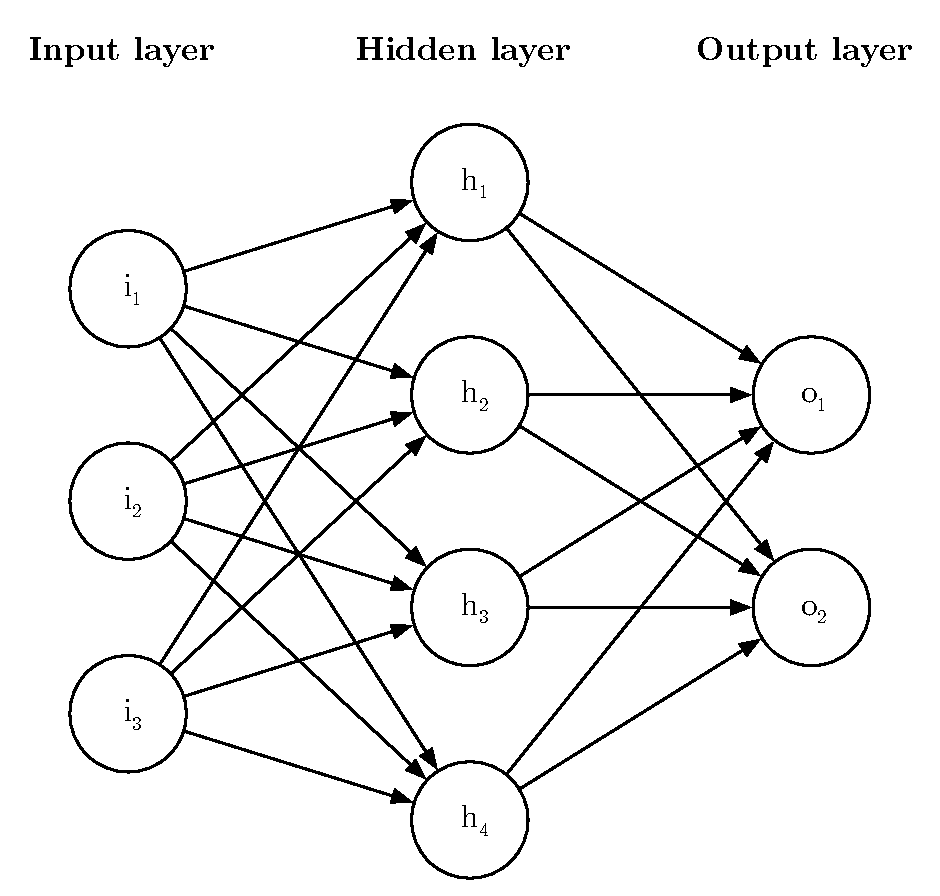
\includegraphics[width=0.6\linewidth]{fig/neural_network.eps}
	\caption{A neural network with one input layer composed of three neurons,
	one hidden layer of 4 neurons, and one output layer with 2 neurons.}
	\label{fig:neural_network}
\end{figure}


In a feedforward neural network, each neuron is connected to every neuron in 
the next layer.  To obtain an output from a given input,
the information will be passed from layer to layer in the following way: 
each neuron computes a weighted sum of the outputs of all neurons in the
previous layer then squashes this weighted sum in an activation function.
\index{activation function} 
Hence, the neuron $h_1$ in the network of Figure~\ref{fig:neural_network}
outputs:
$$ f(w_1i_1 + w_2i_2 + w_3i_3 + b) $$
where $w_1, w_2, w_3$ are the weights \index{weights} corresponding to the
connections between $i_1, i_2, i_3$ and $h_1$; and $b$ is a bias term. 
These weights are the learnable parameters of any neural network and will be 
tuned during training to improve the accuracy of the network. 
The activation function $f(\cdot)$ can be chosen arbitrarily, as long as it 
is differentiable \footnote{This is mostly true, although some activation
functions that have recently been made popular because of their good
performance such as Rectified Linear Units (ReLUs) \cite{relus} are not 
differentiable on all of their domain.}
(so that backpropagation can work, see \ref{nn:training})
but it is the same for all the neurons in the same layer. Some options are
the sigmoid function, the hyperbolic tangent function and sometimes a simple
linear function.\\

The reader might have noticed that using matrices is an efficient way of writing
and executing computations within a neural network. Indeed, one could write
the computation between the input layer and the first hidden layer as: 

$$ h = f_h(iW_{ih} + b_h) $$

\noindent where : 
\begin{itemize}
	\item $h$ is a $1\times n$ vector containing the values of the neurons 
		in the hidden layer
	\item $i$ is a $1\times m$ vector containing the values of the neurons
		in the input layer
	\item $W_{ih}$ is a $m\times n$ matrix containing the weights between
		the input and hidden layer
	\item $b_h$ is the $1\times n$ bias vector 
	\item $f_h$ is the activation function choosen for the hidden layer
\end{itemize}

Similarly, the computation between the hidden layer and the output layer
can be written as:
$$ o = f_o(hW_{ho} + b_o) $$
Hence the full transformation between the input and the output is:
$$ o = f_o\left(f_h(iW_{ih} + b_h)W_{ho} + b_o\right) $$

The example of Figure~\ref{fig:neural_network} is an extremely simple example.
Often, neural networks will be \textbf{wider} (meaning that there are more
neurons per layer) and \textbf{deeper} (meaning that there will be more layers).
This can lead to issues and challenges when training them. The main issue
related to deep neural networks is the vanishing gradient problem, exposed
by Hochreiter \cite{vanishing_gradient}. More generally, adding more 
neurons (or units) increases the possibility of \textbf{overfitting} (see
Section~\ref{sec:regularisation}).

\subsection{Training}
\label{nn:training}
Every neural network is initialised randomly at first, meaning that we will
attribute a random value (that is sampled from a user-defined distribution)
to each weight in the network.\\

If we want to train a network to differentiate a cat from a dog based on a
given set of measurements, we will have to expose it to a large number of examples
of measurements and their associated ground truths \index{ground truth}
(whether the measurements actually correspond to a cat or a dog). This large
number of examples is called the \textbf{training set} $\mathcal{D}$. 
\index{training set} Training is
then performed by alternating feedforward passes (distilling the input through
the network and obtaining the network output) and backpropagation: modifiying 
the weights of the connections between neurons (that will in turn modify 
the network output) until the network output matches the ground truth with 
a good enough accuracy.\\

The forward pass has been explained previously, but the backwards pass, also
called \textbf{backpropagation}, is slightly more complicated.\\

\subsubsection{Loss function}
The first thing we need to improve our network is a number which measures
how far the network output is from the ground truth.
This is exactly what a \textbf{loss function} \index{loss function} does: 
it describes numerically the error between the target and the network output.
One example of a loss function is the mean square error (MSE) \index{MSE} which
is very useful in regression problems:
$$ \mathcal{L}_{\text{MSE}} = \sum\limits_{(x, t) \in \mathcal{D}}\frac{(f(x)-t)^2}{|\mathcal{D}|}$$
where $x$ is a feature vector, $t$ is its corresponding ground truth and $f$
is our model. In
many cases, $f(x)$ and $t$ are vectors, so we may sum or average the loss computed
over components.\\

For classification problems, like the cats and dogs example, one typically uses
a cross-entropy loss which is defined as the following for one sample:
$$-\sum\limits_c t_c\log(f(x)_c)$$
where $c$ is the class index, hence the loss computed over the whole dataset being:
$$\mathcal{L}_{\text{CE}} = \sum\limits_{(x, t) \in \mathcal{D}}
\frac{-\sum\limits_c t_c\log(f(x)_c)}{|\mathcal{D}|}$$
In our cats and dogs example, let us consider that the ground truth for
"cat" corresponds to the output vector $[1, 0]$ and the ground truth for "dog"
corresponds to the output vector $[0, 1]$. If the network predicts $[0.3, 0.7]$
when it is given measurements of a cat, the loss function will equate to :
$$ \mathcal{L} = -(1\log(0.3) + 0\log(0.7)) = -0.47$$
whereas if it had predicted $[0.9, 0.1]$, the loss would have equated to:
$$ \mathcal{L} = -(1\log(0.9) + 0\log(0.1)) = -0.95$$

The experienced reader might already have concluded that since we want to
minimise the loss function, we are confronted with an optimisation problem.

\subsubsection{Backpropagation}
\index{backpropagation}
We will only summarise backpropagation in this section as explaining it in
full is out of the scope of this paper.
The problem at hand is indeed an optimisation problem with the following
parameters:
\begin{itemize}
	\item the objective function, which we want to minimise, is the loss 
		function
	\item the parameters are all the weights of the neural network
\end{itemize}
How can we link the parameters to the objective function? A key requirement
for activation functions and the loss function is that they have to be
\textbf{differentiable}. When this is the case, we can compute the gradient
of the loss function (in other words, the gradient of the error) and 
backpropagate it through the network by using the
chain rule of derivation. The derivative of the loss function can be written
in terms of its partial derivatives with respect to each of the weights
in the network:
$$\nabla\mathcal{L} = \left(
  \frac{\delta\mathcal{L}}{\delta w_1}, 
  \frac{\delta\mathcal{L}}{\delta w_2}, 
  \frac{\delta\mathcal{L}}{\delta w_3}, ...,
  \frac{\delta\mathcal{L}}{\delta w_k}\right) 
$$
Each weight will then be modified by adding a small increment in the direction 
of the gradient:
$$ \Delta w_i = - \alpha \frac{\delta\mathcal{L}}{\delta w_i}$$
where $\alpha$ is the learning rate, a hyperparameter chosen by the designer
of the network that defines the size of the steps to make in the direction
of a smaller error. A high learning rate may accelerate training but could
reduce the chance of finding a global optimum. Reducing the learning rate,
on the other hand, could make the training slower but at the same time 
increase the probability of finding a global optimum.\\

Let us derive the gradient of a weight which connects a neuron in the 
last hidden layer to a neuron in the output layer in the case
where we have a MSE loss:
$$ \Delta w_{oh} = -\alpha\frac{\delta\mathcal{L}}{\delta w_{oh}}$$
which can be expanded using the chain rule:
\begin{equation}
\Delta w_{oh} = -\alpha
\frac{\delta\mathcal{L}}{\delta a_o}
\frac{\delta a_o}{\delta net_o}
\frac{\delta net_o}{\delta w_{oh}}
	\label{eq:chainrule}
\end{equation}
where $net_o$ is the input of neuron $o$ and $a_o$ is the activation value
of neuron $o$.\\

Let us analyse each partial derivative of equation~\ref{eq:chainrule}.
The derivative of the error with respect to the activation is :
$$ \frac{\delta\mathcal{L}}{\delta a_o} = 
\frac{\delta(\frac{1}{2}(t_o-a_o)^2)}{\delta a_o} = -(t_o-a_o)$$
Notice that we injected a $\frac{1}{2}$ factor to the error to simplify 
computations.\\

The derivative of the activation with respect to the input of the neuron is:
$$ \frac{\delta a_o}{\delta net_o} $$
It is simply the derivative of the activation function chosen for
the output layer. Since this derivative will vary depending on the choice
of activation function, we will simply denote is as $f_o'$.\\


The derivative of the neuron input with respect to the weight is
$$ \frac{\delta net_o}{\delta w_{oh}} = \frac{\delta (w_{oh}a_h)}{\delta w_{oh}}
 = a_h$$

Hence we will update a weight between the last hidden layer and the output
layer with:
$$ \Delta w_{oh} = \alpha (t_o-a_o)f_o'(net_o)a_h$$

For weights that connect the penultimate hidden layer to the last layer (in
our case, the input layer to the hidden layer), the error is slightly more 
complicated as it depends on the error of all $k$ neurons in the hidden layer,
and not just of one output neuron. The gradient of such a weight can be
written as:
\begin{equation}
\Delta w_{hi} = -\alpha
	\sum\limits_k \left(
	\frac{\delta\mathcal{L}}{\delta a_k}
	\frac{\delta a_k}{\delta net_k}
	\frac{\delta net_k}{\delta a_h}
	\right)
\frac{\delta a_h}{\delta net_h}
\frac{\delta net_h}{\delta w_{hi}}
	\label{eq:chainrule_further}
\end{equation}
A similar reasoning can be used to unfold equation \ref{eq:chainrule_further}.

Backpropagation uses the fact that activation functions are differentiable to
perform gradient descent. Indeed, the error signal is a surface in a space
of which the dimensionality is equal to the number of parameters in the
network. Gradient descent aims to find the global minimum of this error
surface.\\


\subsubsection{Summary}
To train a neural network, its weights have to be randomly initialised first,
then we show it many examples of the training set, containing measurements and
ground truths. For each of these examples, or samples:
\begin{enumerate}
	\item the feedforward pass computes the network output from the sample
		input data
	\item the network output is compared with the sample output and the
		error signal given by a loss function
		is backpropagated through the network, updating
		all the weights
\end{enumerate}

\subsection{Overfitting and regularisation}
\label{sec:regularisation}

\section{Recurrent neural networks}
There is one limitation to feedforward neural networks which can be particulary
critical for some applications. Very often, having an output mapped to a 
single input is not enough. For example, in problems where samples are organised
in a timeline and dependent on each other, only seeing one input at a time
does not provide enough information. If one wants to predict the weather
temperature in the next hour, it would be useful to know more than only the
last ground truth value to identify a potential trend. One 
could input a fixed-size window of the previous time steps to the network,
but this approach limits the scope of available "memory" and could dramatically
increase the complexity of the model.\\

One solution to this problem is the use of recurrent neural networks.
A feedback loop such as the one shown in Figure~\ref{fig:rnn}a, also called
a recurrent connection, means that the layer at the receiving end of the
recurrent connection will receive as input not only the value of the previous
layer at time $t$, but also the value of the layer at the giving end of the 
recurrent connection at time $t-1$. This allows information to \textit{live}
throughout time steps.\\

A recurrent connection, however, poses evident issues for the backpropagation
algorithm since the depth of the neural network can become theoretically
infinite.  A common way of training and visualising recurrent neural networks 
is to unroll them for a given, finite amount of time steps (see 
Figure~\ref{fig:rnn}b).  The error signal can then be computed
for the output value at each time step, and backpropagated through all the
previous input values that affected its computing.\\

\begin{figure}[]
	\centering
	\subfloat[][A recurrent connection]{\qquad
		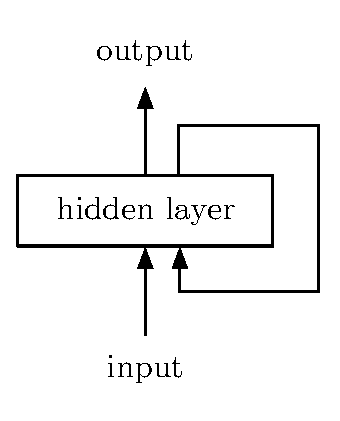
\includegraphics[width=0.1515\linewidth]{fig/recurrent_neural_network.eps}\qquad}
	\qquad
	\subfloat[][An unrolled recurrent neural network]{
		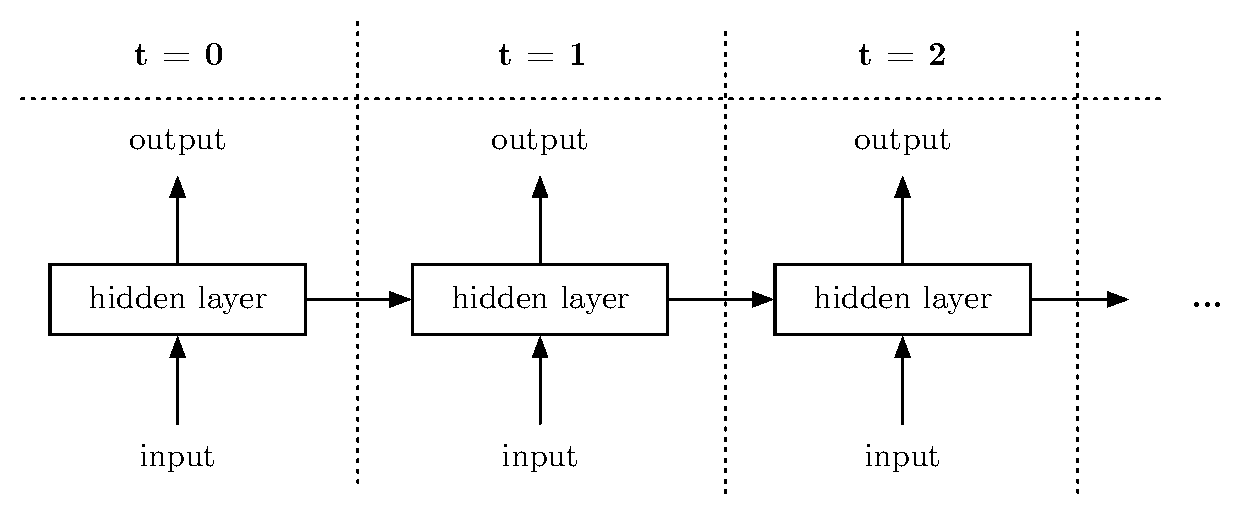
\includegraphics[width=0.6\linewidth]{fig/recurrent_neural_network_unrolled.eps}}
	\caption{Recurrent neural networks}
	\label{fig:rnn}
\end{figure}

\subsection{Long Short-Term Memory (LSTM)}
One major issue encountered when using recurrent neural networks is that they
are famous for being unstable. Very often, at some point, training will diverge
and will never reach a satisfying optimum. Several solutions have been presented
to counter this unstability, one of them being Long Short-Term Memory (LSTM)
cells \cite{lstm}. \\

\begin{figure}
	\centering
	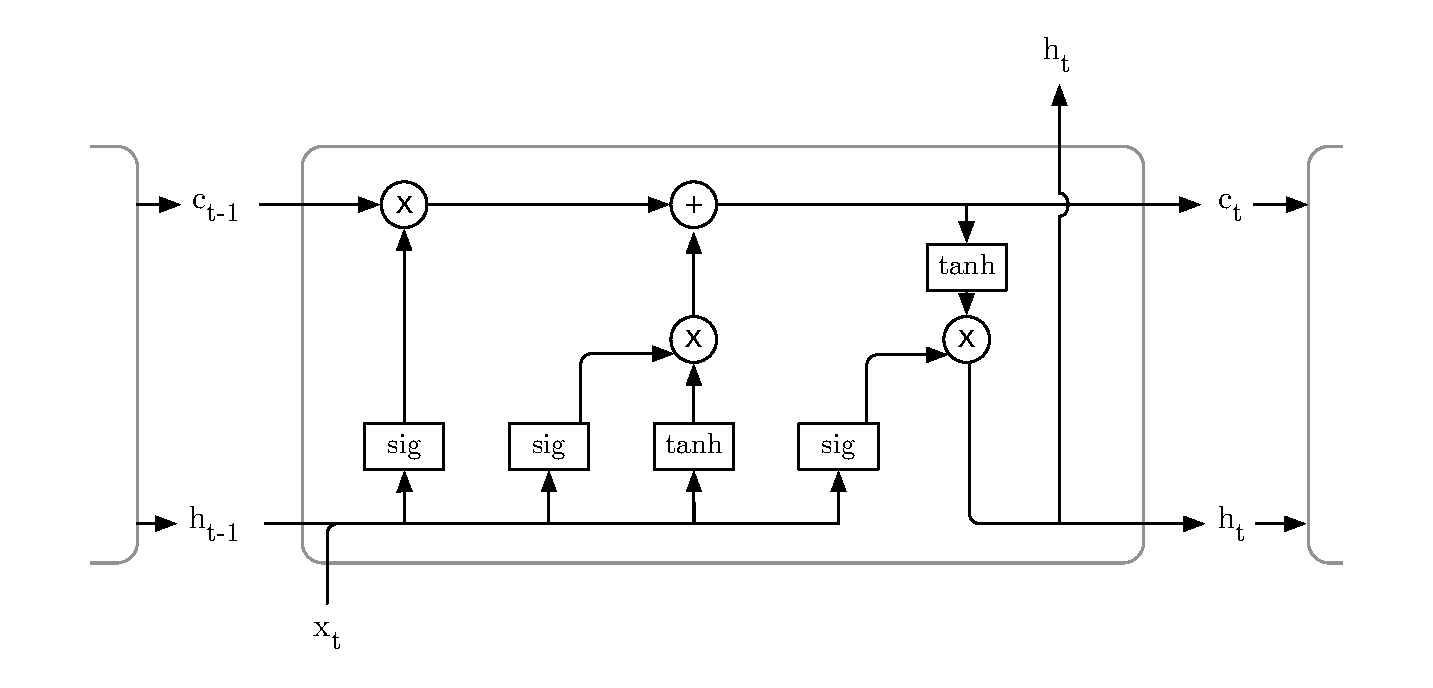
\includegraphics[width=0.8\linewidth]{fig/lstm.eps}
	\caption{The internals of a LSTM cell. Circles represent element-wise
	operations (arrows carry vectors). \framebox{sig} and 
	\framebox{tanh} are layers. $c_t$ is the memory cell.}
	\label{fig:lstm}
\end{figure}

Instead of carrying to the next timestep only the hidden state (which is also
the output of the cell), LSTMs also carry what is called the
\textit{memory cell} $c_t$ which isn't used as output. This memory cell is 
able to handle longer term memory management by using \textit{gates} to 
access and modify it. All gates receive a concatenation of the previous hidden
state $h_{t-1}$ and the new input vector $x_t$. They feed this input through a
sigmoid layer (\framebox{sig})to an element-wise multiplication. There are 
three in total, as they can be seen from left to right on Figure~\ref{fig:lstm}:
\begin{enumerate}
	\item the \textit{forget gate} is the first one. It will multiply each
		value in the memory cell by a value in $[0, 1]$, keeping only
		the values it considers useful.
	\item the \textit{update gate} is the second one and it chooses which
		ones of the outputs of the first \framebox{tanh} layer will
		make their way to the memory cell.
	\item the \textit{output gate} is the last one and decides what parts
		of the memory cell make it to the output.
\end{enumerate}

\todo{universal function approximators}



\chapter{Reinforcement Learning}
\begin{quotation}
\noindent ``\emph{quote}''
\begin{flushright}\textbf{auteur, date}\end{flushright}
\end{quotation}

\vspace*{0.5cm}

\section{Machine Learning}
One could trace back the birth of the machine learning idea to Alan Turing's 
seminal paper, \textit{Computing Machinery and Intelligence} 
\cite{turing1950computing}. Although the computer science context around his
work was largely inexistent (at least compared to today), Turing already felt
the need to think of ways to transcend the fixed set of rules a computer had
to interpret and execute. As computer science grew, and as the field of
artificial intelligence went through its ebbs and flows throughout the years,
machine learning evolved from an idea to a prolific field of research, and
some of its topics saw massive application into real world domains.\\

The most popular and widely used machine learning algorithms and techniques
usually come from what we call supervised and unsupervised machine learning.
The broad goal of supervised machine learning is to find a function that maps
some input vector $x$ to some output vector $y$. One example of this would be
to try to categorise patients that either have or don't have some disease. 
The input vector $x$ could contain measurements such as blood pressure, the 
quantity of a given substance in the patient's blood, etc. The output vector
$y$ would be either $[0]$ if the patient is ill, and $[1]$ if the patient is
not.\\

If we could find a function mapping $x$ to $y$, we could predict to some
level of accuracy if a patient is ill or not by only knowing $x$. The general
algorithm for finding such a function is to define a model which has
\textit{learnable parameters}; that is values which impact the output of the
function, and to perform \textbf{training}. The process of training is to
sample one data point from a \textbf{training set}, containing pairs of input
vectors and output vectors. We then feed the input vector to our model, compare
the output that we get from the model with the output we are supposed to get,
and tune our learnable parameters so to minimise the error between the model
output and the correct output. We repeat this process, showing many samples
of the training set to our model until it reaches a good enough accuracy.

Unsupervised learning, although different from supervised learning as the
training sets usually do not have output vectors, is more about finding
structure in the dataset; but we can assume for the sake of this point that
the process is largely the same.\\

To the critical reader, unsupervised machine learning and supervised machine
learning might sound like fancy names for statistics; and one could argue that
they are indeed. Perhaps a slightly more interesting topic of machine learning
would be \textbf{reinforcement learning}. In this setting, we train an agent, 
which is situated in an environment, to perform actions that will maximise
a reward given by the environment.\\

This process works by letting the agent interact with the environment for many
sessions, until it figures out what actions, and what sequences of actions lead
to high rewards. This is the training process of a reinforcement learning agent.
One example of this is the CartPole problem \cite{barto-cartpole} where the
agent controls a cart on which a pole is balanced. The goal is to keep the
pole balanced for as long as possible by nudging the cart left or right. The
agent receives the position of the cart, the velocity of the cart, the pole
angle and the pole velocity at tip as a state observation from the environment,
and has to push the cart either left or right. The agent will first perform
randomly, but sooner or later, it will figure out how to balance the pole.\\

One common issue between all of the techniques described above is that once
training is over, the behaviour of the trained agent or model will not change
or adapt once the conditions, or some intrinsic parameters of the problem
change. If we present the CartPole agent with a pole that is twice as heavy,
or twice as long as the one it has been trained with, it will likely fail to 
balance the pole. We have taught an agent how to solve one task, but we have
not taught it to learn how to solve a task. The agent that has been trained is
not a learning agent. This thesis will explore ways to teach an agent to learn
to solve tasks.

\section{The reinforcement learning problem}
A reinforcement learning setting sees two main components interact : the agent
and the environment. The environment can be in several states which the agent
can observe (for example in the CartPole problem : the cart can be in several 
positions and have different velocities, and the pole has similar 
characteristics). In some problems, the agent might not be able to observe the
full state of the environment.\\

The agent chooses actions based on its knowledge of the state of the
environment. These actions might (and often do) alter the state of the
environment, but will also generate a reward. In the CartPole problem, the 
reward is +1 every tick the pole is above a certain angle, 0 otherwise.\\

With this simple setting, of which a diagram is shown in Figure~\ref{fig:rl},
we can design algorithms that can be trained to solve a huge variety of tasks
without ever having to include task-specific logic to the algorithm.

\begin{figure}[]
	\centering
	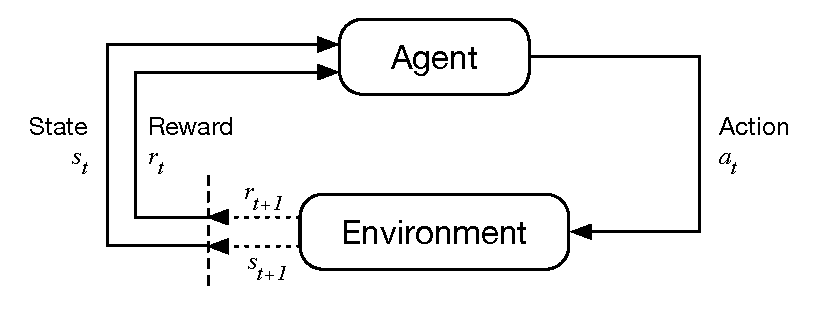
\includegraphics[width=0.65\linewidth]{fig/rl.eps}
	\caption{The setting of a reinforcement learning problem 
		\cite{suttonbarto}}
	\label{fig:rl}
\end{figure}

\subsection{Markov Decision Processes}
A reinforcement learning problem can be formally defined as a Markov 
Decision Process (MDP) \index{MDP} characterised by :
\begin{itemize}
	\item a set of states $\mathcal{S}$
	\item a set of actions $\mathcal{A}$
	\item a transition function 
		$T(s, a, s') = P(s_{t+1} = s' \mid s_t = s, a_t = a)$
	\item a reward function 
		$r(s, a, s') = \mathbb{E}
		 [r_{t+1} \mid s_t = s, a_t = a, s_{t+1} = s']$
\end{itemize}
For the rest of this paper, we will consider that the transition function is
deterministic.\\

The goal of reinforcement learning is for the agent to select, in any state it
can be in, the action that will lead it to the highest expected reward :

\begin{equation}
\mathbb{E}[r] = r_t + \gamma r_{t+1} + \gamma^2 r_{t+2}^2 + ... =
 \sum\limits_{i=0}^\infty \gamma^i r_{t+i}
\end{equation}

\noindent with the discount factor \index{discount factor} $\gamma \in [0, 1[$.
The discount factor allows one to tune the agent's behaviour on the
short-term/long-term spectrum. A discount factor $\gamma=0$ would mean that the
agent maximises its expected reward for the next transition only whereas a
discount factor close to one will favour behaviour that maximises long-term
reward, even if one action leads to a poor reward at first.\\

\subsection{Policy}
The agent uses a policy $\pi(a \mid s)$ which describes a probability
distribution over the action set $\mathcal{A}$, determining the probability of
selecting action $a_i$ from state $s_i$. This policy is 
\textbf{deterministic} if and only if :
\begin{equation}
\forall\, s \in \mathcal{S},\; \exists\, a \in \mathcal{A} : \pi(a \mid s) = 1
\end{equation}
\noindent Otherwise, the policy is \textbf{stochastic}.

\section{An example : the 2-armed bandit problem}





\part{Meta Reinforcement Learning}
\chapter{Learning to learn}
\begin{quotation}
\noindent ``\emph{quote}''
\begin{flushright}\textbf{author}\end{flushright}
\end{quotation}

\vspace*{0.5cm}

Developing and tuning algorithms to find the optimal strategy to solve a
reinforcement learning problem is hard. Some of the challenges one meets are:
\begin{itemize}
	\item the tradeoff between exploration and exploitation
	\item designing a strategy that allows for versatile training
	\item choosing hyperparameters \todo{define} that make the strategy
		optimal considering the reinforcement learning problem at hand
\end{itemize}

Let us consider the problem of learning a simple bandit problem with dependent
arms. Say, for example, that a bandit has two arms, each of which producing
a reward according to a Bernoulli distribution with the following parameters :
$$ \begin{cases} P(r \mid \text{arm}_1) = p_b \\ 
P(r \mid \text{arm}_2) = 1 - p_b  \end{cases} $$
where $P(r \mid \text{arm}_1)$ is the probability of arm 1 to generate a reward
and $0 \leq p_b \leq 1$ is the parameter of the bandit problem. One way to
solve this problem would be to use the $\epsilon$-greedy strategy. This
strategy keeps an average of the reward of each earm and chooses the next
action the following way : choose the action with the best average
reward so far with probability $(1-\epsilon)$, otherwise choose a random action.
This raises the question about choosing $\epsilon$. Choosing a low $\epsilon$
encourages exploitation but we have a higher chance of wrongly estimating $p_b$.
Choosing a high $\epsilon$ doesn't allow the agent to perform optimally once
its knowledge about the parameters of the problem is likely to be optimal.
Moreover, we could choose a variable $\epsilon$, high at first but slowly
converging to 0, but we then are faced with the choice of another
hyperparameter : the number of steps over which $\epsilon$ should be annealed.\\

One could propose using a more advanced method, and there are many. Multi-armed
bandits have been heavily studied and to this day, several algorithms exist to
solve the kind of bandit problems defined above very quickly - i.e. to explore
just enough to implicitly learn $p_b$ so to exploit the best arm as much as
possible. Examples of these algorithms are the Gittins indices algorithm
\cite{Gittins79banditprocesses},
UCB \cite{Auer:2002:FAM:599614.599677} and Thompson sampling
\cite{thompson1933}.\\

The obvious problem here is that we can always choose to manually design more
and more sophisticated techniques and to tune more perfectly their parameters,
but could we not instead use reinforcement learning to do this for us instead?\\

Recently, Wang et al. \cite{learningtorl} and Duan et al. \cite{fastrlviaslowrl}
proposed the idea of using reinforcement learning to learn an algorithm which
deploys an optimal strategy for a class of problems sharing a similar structure.
We will use the name "meta-RL" or meta-learning for this technique, as proposed 
by Wang et al. Generally, we will call the learned algorithm the inner
algorithm, and the algorithm that learns to learn the outer algorithm.\\

\begin{figure}
	\centering
	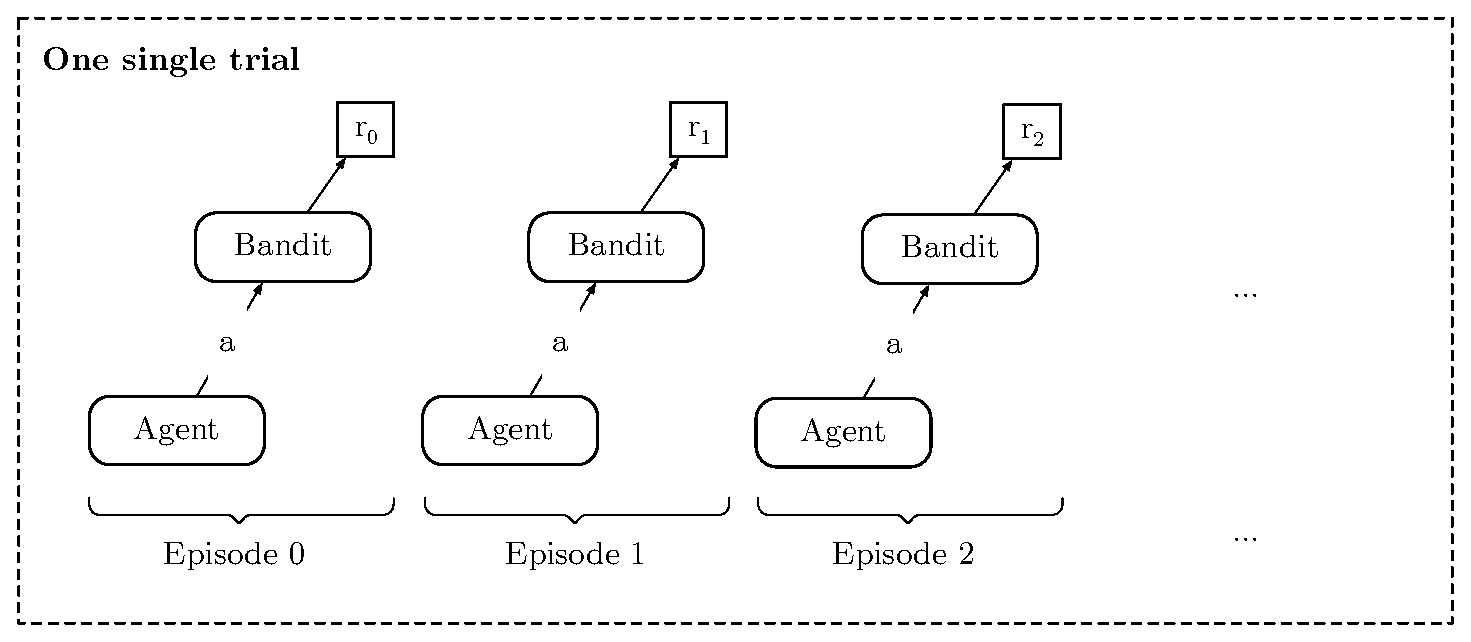
\includegraphics[width=0.7\linewidth]{fig/normal_bandit_training.eps}
	\caption{A classic training sequence to learn a bandit problem. One
	manually designs a strategy which inspects the reward obtained at 
	the end of an episode and evaluates the performance of the action
	taken accordingly. The strategy then updates the policy.}
	\label{fig:normal_bandit_training}
\end{figure}

In classic reinforcement learning (see Figure~\ref{fig:normal_bandit_training}),
the goal of the agent is to maximise its
expected reward for each episode; for this, we let the agent play several
episodes, choosing actions according to a policy which is learned over time, 
but of which the learning process is manually defined by a strategy (Gittins,
UCB, ...) hoping that the agent will yield high rewards as fast as possible.
The part of this process we are interested in is the hand-designed updating of
the policy inbetween episodes.\\

As stated at the beginning of this chapter, designing strategies to learn
policies is a hard task and can demand a sensitive tuning of parameters.
Instead of manually designing ways to make the agent succeed faster, in meta-RL,
the agent plays a trial of several episodes of the same problem and has to
maximise its expected reward across all episodes of a trial (see 
Figure~\ref{fig:meta_bandit_training}). This will incentivize the agent
to understand the structure of a problem and develop a strategy that allows it 
to estimate the parameters of the problem as fast as possible.\\

\begin{figure}
	\centering
	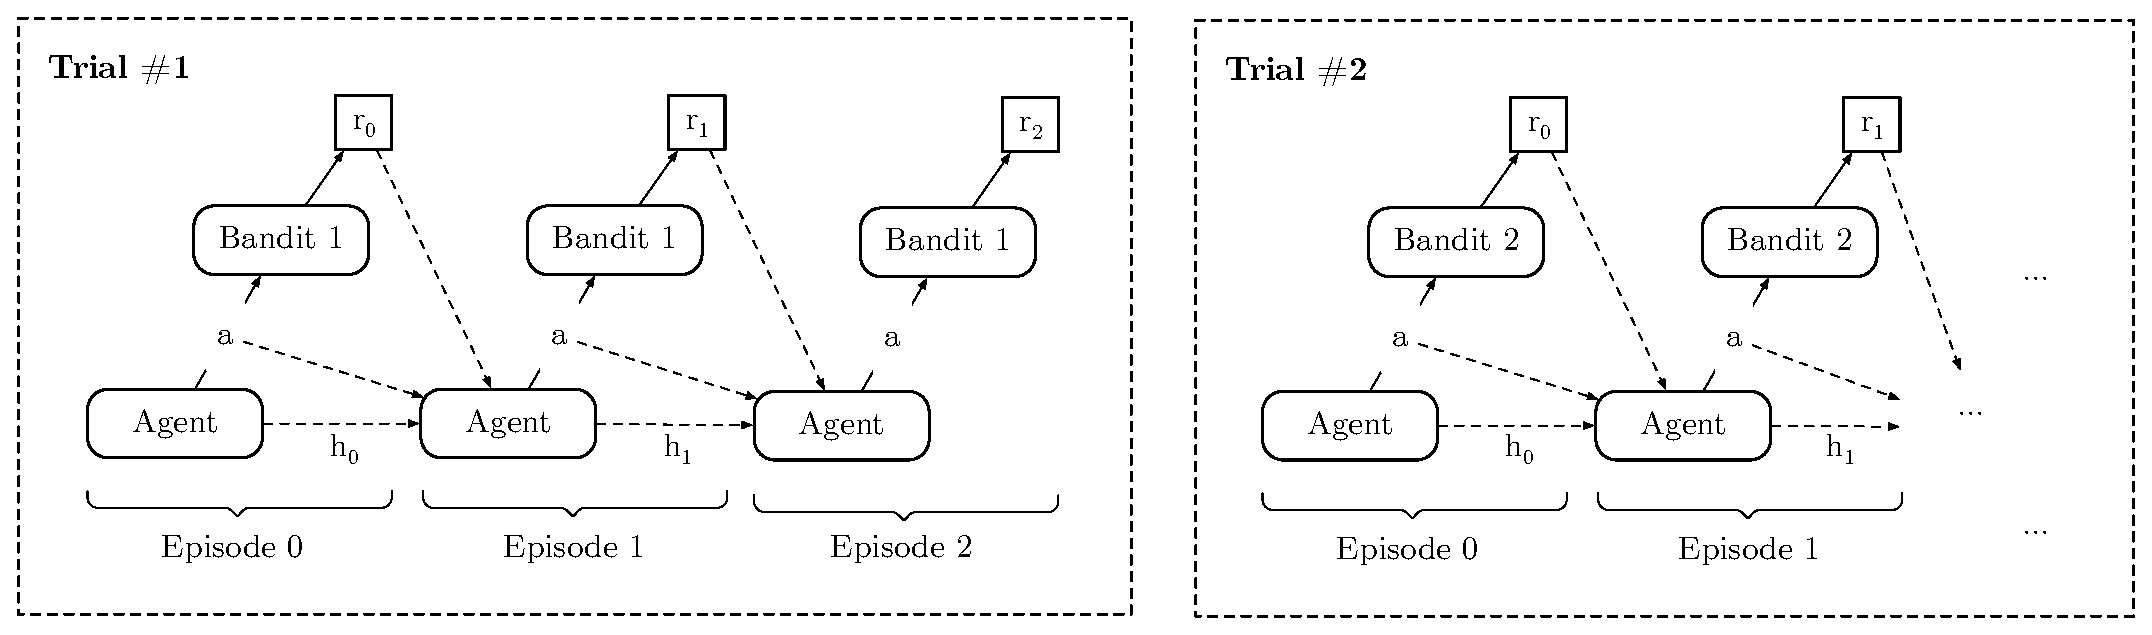
\includegraphics[width=\linewidth]{fig/meta_bandit_training.eps}
	\caption{The training sequence for a meta-RL agent on a bandit problem.
	In this case, the agent is left to play several episodes on its own
	without changing its weights. It is only when a trial ends that the
	outer algorithm evaluates the rewards of all episodes in the trial and
	updates the weights of the inner algorithm so that it increases its
	chances of having a better reward across all episodes. For trials of 
	two episodes such as the one presented in this figure, the outer
	algorithm forces the inner algorithm to learn the problem in 
	two episodes.}
	\label{fig:meta_bandit_training}
\end{figure}

In our manually designed strategies, we use previous actions and rewards
to update the policy and make it better. Similarly, in order to
make meta-RL work, the agent has to receive as input the previous reward
and the action that led to that reward, but it also needs to carry on some
sort of memory of past actions and rewards.\\


\begin{figure}
	\centering
	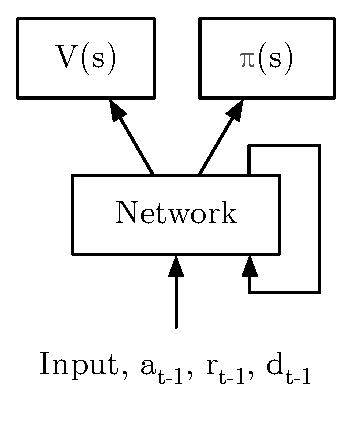
\includegraphics[width=0.2\linewidth]{fig/a2c_meta.eps}
	\caption{The meta-learning A2C agent}
	\label{fig:a2c_meta}
\end{figure}

\begin{figure}
	\centering
	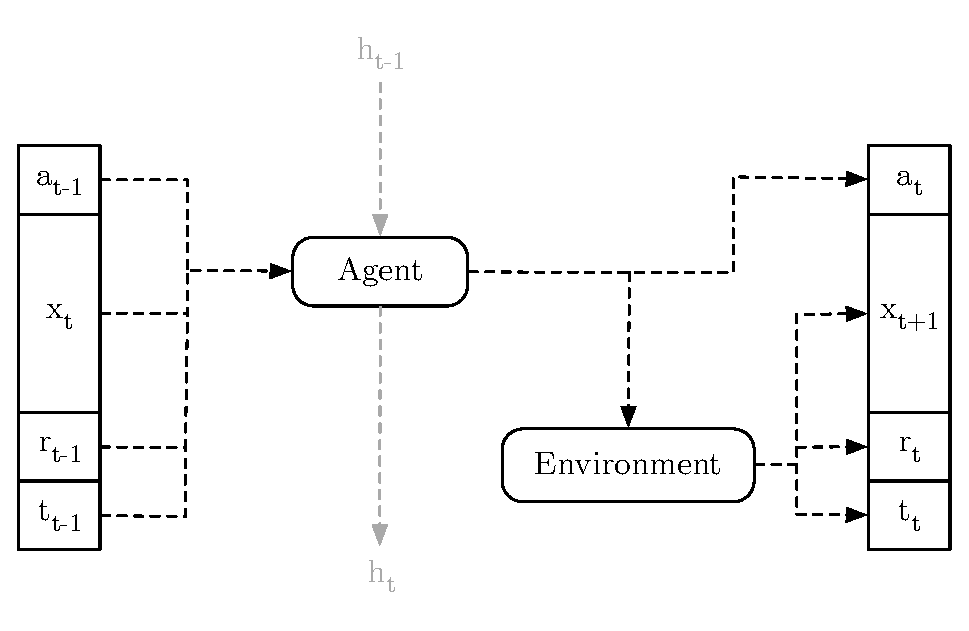
\includegraphics[width=0.6\linewidth]{fig/meta_rl_timestep.eps}
	\caption{An unrolled timestep in the meta-RL training setting. At each
	timestep, the agent receives an observation of the state of the
	environment as well as the previous action taken, the associated reward,
	and the termination flag. It also receives its previous hidden state
	if and only if the previous timestep was part of the same trial (this
	could still mean that the last timestep was from a different episode
	which just terminated)}
	\label{fig:meta_rl_timestep}
\end{figure}

The general setup presented by Wang et al. uses a recurrent neural network of
which the weights, once trained "slowly" over several trials of multiple
episodes, will encode the "fast" training policy.
Figure \ref{fig:a2c_meta} shows the meta-learning A2C agent presented in Wang
et al. \cite{learningtorl}. There are two differences to note compared to
Figure~\ref{fig:a2c}: the first one is the recurrent connection, and the
second one is the set of values we input to the agent at each time step. In
addition to the state of the environment, we add the previous action, 
previous reward and a termination flag which is set to 1 when an episode
has reached a terminal state; 0 otherwise.\\

It is important to emphasize on the fact that the agent passes on its hidden
state between different episodes of the same trial (and if episodes last for
more than one timestep, between timesteps as well), but \textbf{not} between
trials (see Figure~\ref{fig:meta_bandit_training}).
The reason why the inter-episode connection is needed is because
the agent might want to deploy a different policy given the results of 
previous episodes as it has to optimise its expected reward across multiple
episodes.

\todo{Talk about bandit results?}

\section{Meta-learning CartPole}
\label{section:setting}
We will study the performance of meta-learning on various distributions of 
the CartPole problem. The CartPole environment describes a cart, rolling on 
a frictionless rail. A pole is attached to the cart and has to be kept balanced
above the cart for more than 195 timesteps by also keeping the cart within a 
defined section of the rail. The agent has two actions at its disposal: nudge
the cart left or right. The observation of the state is a 4-valued vector 
containing the position of the cart, its velocity, the angle of the pole and
the velocity of the pole at its tip. At each time step, the environment emits
a reward of +1; so if the agent keeps the pole and the cart in their 
respective acceptable ranges for 20 timesteps, it will receive a total reward
of 20.\\
\todo{figure}

\subsection{Generating a distribution of CartPole problems}
To generate a distribution of similar, yet different CartPole problems, we
will play with two different parameters.

\paragraph{Permutations} In standard reinforcement learning, the state
observation vector is always ordered, meaning that each component of the vector
always represents the same value (in CartPole for example, the first component
represents the position of the cart). We can generate a set of $4! = 24$
CartPole problems where for each problem, the state observation vector is
permutated with problem-unique permutation. This means that the agent will
receive a vector of 4 values without knowing which is which.

\paragraph{Actions inversion} We will also introduce the inversion of the
agent's actions. Just like the input vector, the policy output is ordered
(the first component of the policy corresponds to the first action which is
always the same). We will study how inverting actions affects training : instead
of always associating the first component of the policy vector with going left,
we will duplicate each of the 24 problems stated above by inverting the left
and the right action. This adds up to a distribution of 48 CartPole problems.

\begin{figure}
	\centering
	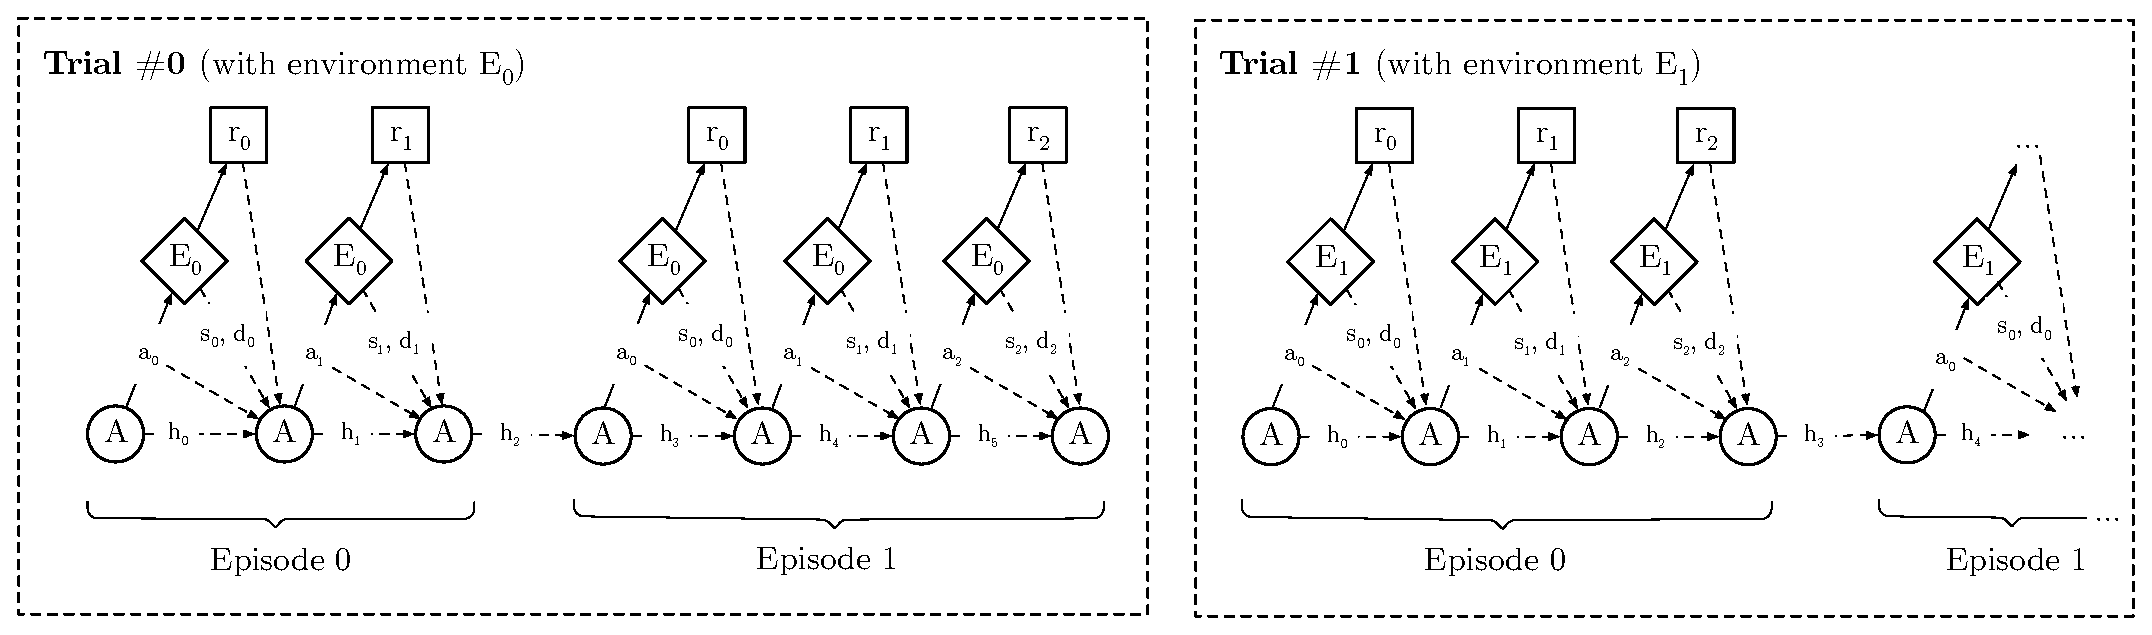
\includegraphics[width=\linewidth]{fig/meta_cartpole.eps}
	\caption{Meta-learning for multi-timestep episodes. A is the agent,
	$E_0$ is the problem selected from the distribution for the duration
	of a trial, $s_t$, is the state of the environment, $r_t$, the reward,
	$a_t$ is the chosen action, $d_t$ the terminal state and $h_t$ is
	the hidden state at timestep $t$. Note that the same environment is
	used throughout all episodes of the same trial.} 
	\label{fig:meta_cartpole}
\end{figure}

\subsection{Agent architecture}
Our agent is an A2C agent built as described in Figure~\ref{fig:a2c_meta}.
The input vector is a concatenation of the state observation, the previous
action taken, the reward obtained at the previous timestep and the termination
flag :
$$ i = [s_t, a_{t-1}, r_{t-1}, d_{t-1}] $$
The action taken is converted to a one-hot encoding (converting the action
index into a vector of length $|A|$ containing zeros except a single 1 at the
index of the action). This vector is then fed to a LSTM sized at 48 hidden
units, followed by two branches :
\begin{enumerate}
	\item a fully connected softmax layer with $|A|$ units (the policy
		output). Actions are selected by sampling according to the
		distribution defined by the policy, rather than by taking the
		action with the highest probability.
	\item a fully connected linear layer with 1 unit (the value output).
\end{enumerate}
The loss of the A2C agent is the following : 
$$ \mathcal{L} = \beta_v \mathcal{L}_v + \beta_p \mathcal{L}_p - \beta_e 
 \mathcal{L}_e $$
where $\mathcal{L}_v$ is the value loss : 
$$ \mathcal{L}_v = (R_{t-1} - V(s_t))^2$$
$\mathcal{L}_p$ is the policy loss : 
$$ \mathcal{L}_p = \pi(a_t \mid s_t) (R_t - V(s_t))$$
$\mathcal{L}_e$ is the entropy regularisation : 
$$ \mathcal{L}_e = \sum\limits_{a \in A}\pi(a \mid s_t)\log(\pi(a \mid s_t))$$
and $\beta_v = 0.5$, $\beta_p = 1$, $\beta_e = 0.05$. An update is performed
once after every trial using Adam \cite{adam} with a learning rate of 0.001.\\

Unless stated, the discount factor used in all experiments is $\gamma=0.9$. 




\chapter{Knowledge gain across episodes}
\begin{quotation}
\noindent ``\emph{Failure is simply the opportunity to begin again,
	this time more intelligently.}''
\begin{flushright}\textbf{Henry Ford}\end{flushright}
\end{quotation}
\vspace*{0.5cm}

\section{Meta-learning CartPole setting}
\label{sec:setting}
We will now go beyond the bandit experiments presented in Wang et al. 
\cite{learningtorl} and Duan et al. \cite{fastrlviaslowrl} and extend the study 
of the performance of meta-learning on multi-timestep
episodes; and for that purpose, we will use various distributions of 
the CartPole problem. The CartPole environment describes a cart, rolling on 
a frictionless rail (see Figure~\ref{fig:cartpole_illustration}). 
A pole is attached to the cart and has to be kept balanced
above the cart for more than 195 timesteps by also keeping the cart within a 
defined section of the rail. The agent has two actions at its disposal: nudge
the cart left or right. The observation of the state is a 4-valued vector 
containing the position of the cart, its velocity, the angle of the pole and
the velocity of the pole at its tip. At each time step, the environment emits
a reward of +1; so if the agent keeps the pole and the cart in their 
respective acceptable ranges for 20 timesteps, it will receive a total reward
of 20.\\


\subsection{Generating a distribution of CartPole problems}
To generate a distribution of similar, yet different CartPole problems, we
will play with two different parameters.

\paragraph{Permutations} In standard reinforcement learning, the state
observation vector is always ordered, meaning that each component of the vector
always represents the same value (in CartPole for example, the first component
represents the position of the cart). We can generate a set of $4! = 24$
CartPole problems where for each problem, the state observation vector is
permutated with a unique permutation. This means that the agent will
receive a vector of 4 values without knowing which is which.

\paragraph{Actions inversion} We will also introduce the inversion of the
agent's actions. Just like the input vector, the policy output is ordered
(the first component of the policy corresponds to the first action which is
always the same). We will study how inverting actions affects training : instead
of always associating the first component of the policy vector with going left,
we will duplicate each of the 24 problems stated above by inverting the left
and the right action. This adds up to a distribution of 48 CartPole problems.\\

Figure~\ref{fig:meta_cartpole} shows how the single-timestep framework
presented in Figure~\ref{fig:meta_bandit_training} adapts to episodes
with multiple timesteps.

\begin{figure}[H]
	\centering
	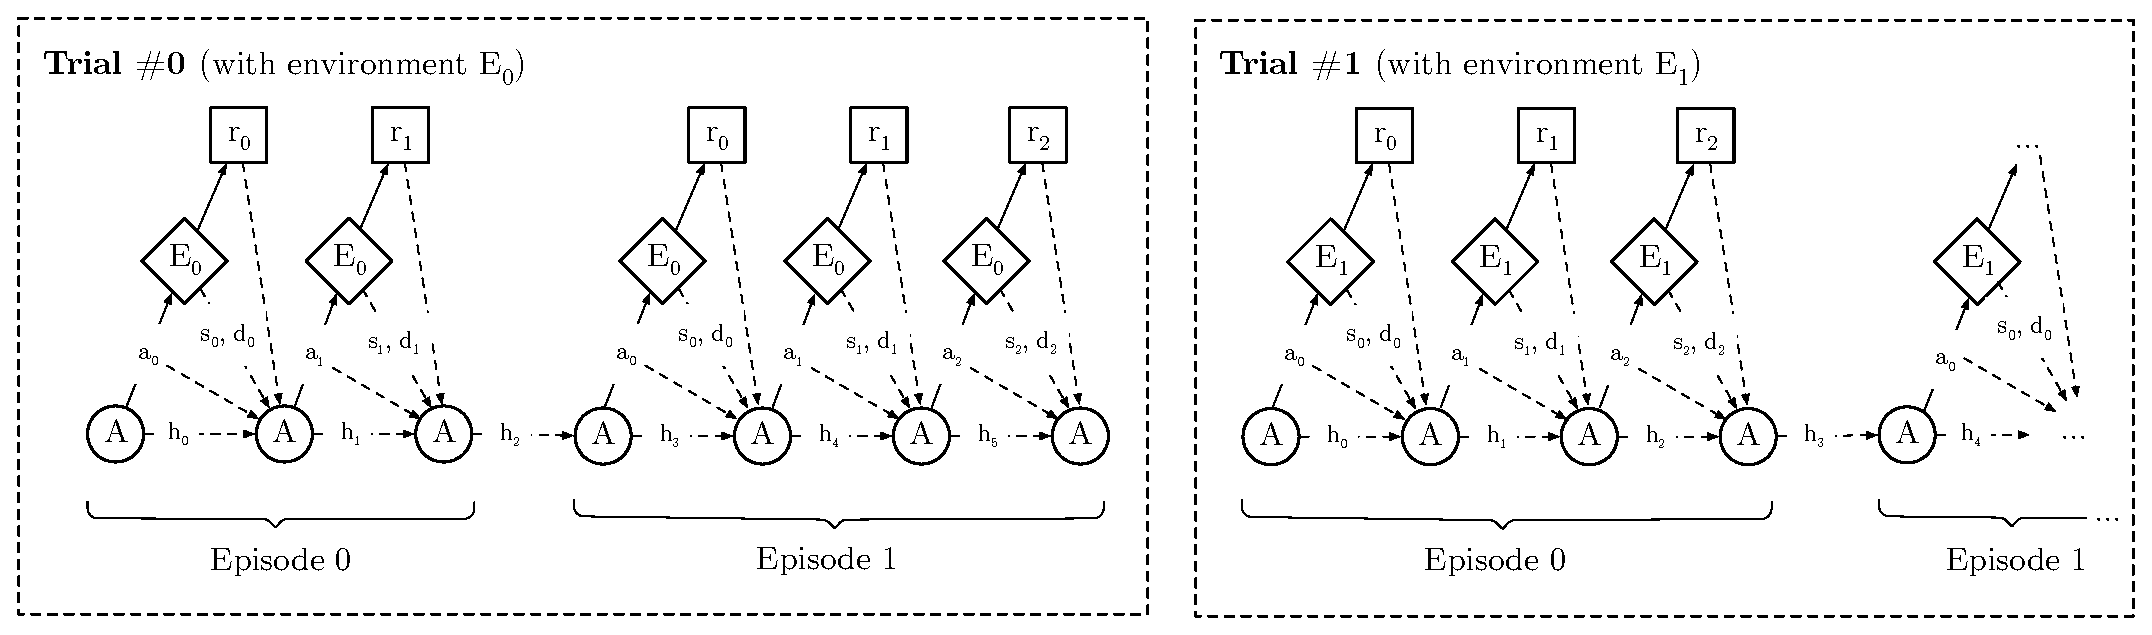
\includegraphics[width=\linewidth]{fig/meta_cartpole.eps}
	\caption{Meta-learning for multi-timestep episodes. A is the agent,
	$E_0$ is the problem selected from the distribution for the duration
	of a trial, $s_t$, is the state of the environment, $r_t$, the reward,
	$a_t$ is the chosen action, $d_t$ the terminal state and $h_t$ is
	the hidden state at timestep $t$. Note that the same environment is
	used throughout all episodes of the same trial.}
	\label{fig:meta_cartpole}
\end{figure}

\section{Performance gain when playing multiple episodes}

We will first and foremost analyse how a reinforcement learning agent 
performs when it is confronted to playing a single episode of one of the 
CartPole problems. We will train the agent on a distribution of 18 permutations
(shown in Table~\ref{tab:20perms}), at first without inverting the agent's
action.\\

\begin{table}
	\centering
	\caption{State permutations used for training and testing}
	\label{tab:20perms}
	\stackunder[5pt]{\small (a) Training distribution}{
		\bgroup
		\def\arraystretch{1.5}
		\begin{tabular}{c|c|c}
			[0, 1, 2, 3] & [1, 0, 2, 3] & [2, 0, 1, 3] \\
			\hline
			[0, 1, 3, 2] & [1, 0, 3, 2] & [2, 0, 3, 1] \\
			\hline
			[0, 2, 1, 3] & [1, 2, 0, 3] & [2, 1, 0, 3] \\
			\hline
			[0, 2, 3, 1] & [1, 2, 3, 0] & [3, 0, 1, 2] \\
			\hline
			[0, 3, 1, 2] & [1, 3, 0, 2] & [3, 0, 2, 1] \\
			\hline
			[0, 3, 2, 1] & [1, 3, 2, 0] & [3, 1, 0, 2] 
		\end{tabular}
		\egroup
	}
	\stackunder[5pt]{\small (b) Testing distribution}{
		\quad\quad
		\bgroup
		\def\arraystretch{1.5}
		\begin{tabular}{c}
			[2, 1, 3, 0] \\
			\hline
			[2, 3, 0, 1] \\
			\hline
			[2, 3, 1, 0] \\
			\hline
			[3, 1, 2, 0] \\
			\hline
			[3, 2, 0, 1] \\
			\hline
			[3, 2, 1, 0]
		\end{tabular}
		\egroup
		\quad\quad
	}
\end{table}

As a control experiment, we first need to check whether the agent can learn
to discover which permutation of the state has been selected and to keep the
pole balanced within one single episode. Surprisingly, as shown in 
Figure~\ref{fig:20perms1ep_training}, the agent quickly manages to reach
a very good performance level, only failing a small percentage of the time.\\

\begin{figure}[H]
	\centering
	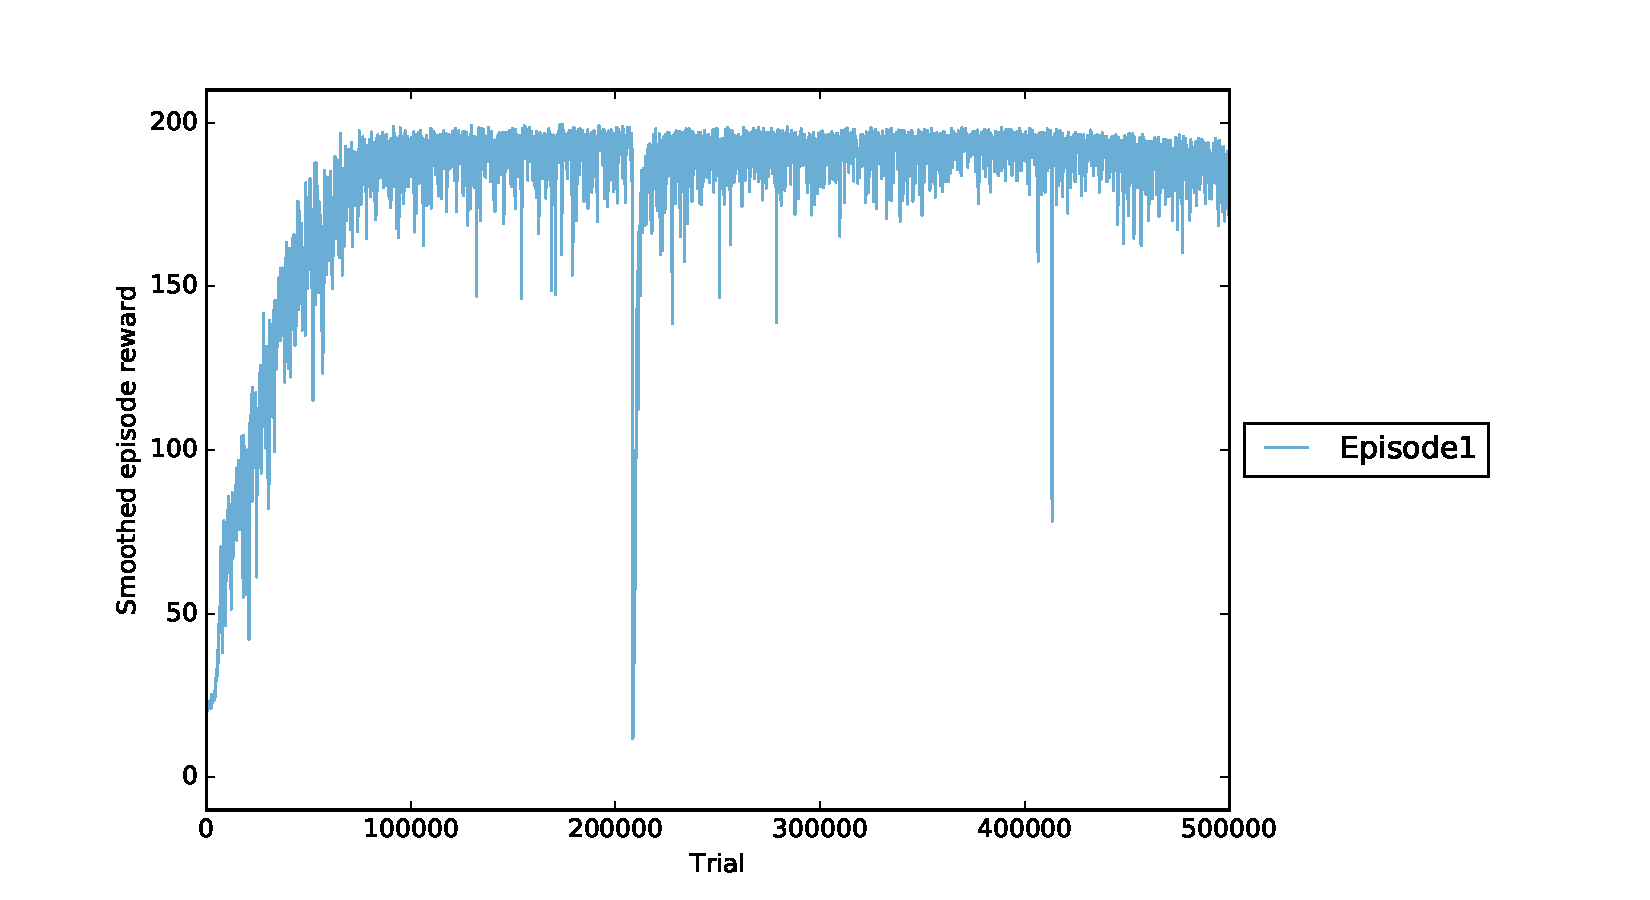
\includegraphics[width=0.9\linewidth]{fig/20perms1ep_training.pdf}
	\caption{Training of an agent on trials of 1 episode. The curve
	shows a moving average over 200 trials.}
	\label{fig:20perms1ep_training}
\end{figure}

When the agent is trained on trials of 2 episodes, we expect that its
performance will improve (however good it already is). Looking at the graph 
of Figure~\ref{fig:20perms2ep_training}, we can only deduce two things : 
\begin{enumerate}
	\item the performance of the first episode of every trial drops 
		significantly compared to trials of one episode;
	\item the performance of the second episode of every trial matches
		closely the performance of single-episode trials.
\end{enumerate}

\begin{figure}[H]
	\centering
	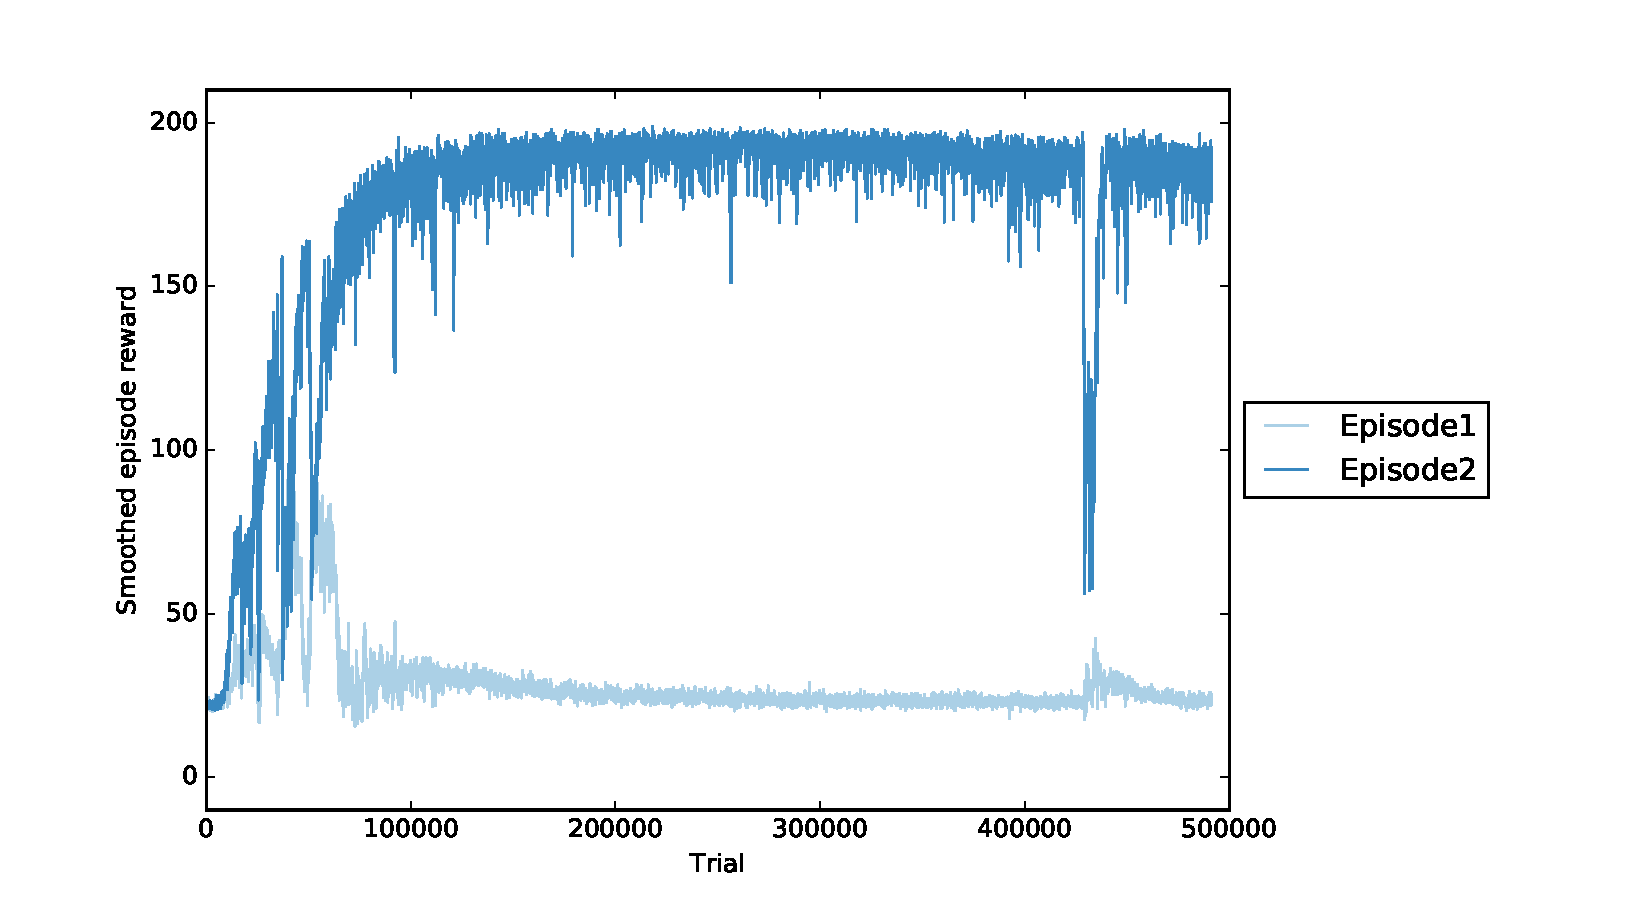
\includegraphics[width=0.9\linewidth]{fig/20perms2ep_training.pdf}
	\caption{Training of an agent on trials of 2 episodes}
	\label{fig:20perms2ep_training}
\end{figure}

The first of these considerations will be addressed in
chapter~\ref{chap:reward_structure}. Let us analyse the second one in more detail
as the average reward graph doesn't give us enough insight in the final
reward distributions.\\


Let us compare the final reward distribution for the only episode of 
single-episode trials and for the second episode of dual-episode trials.
For now, we are not interested in the reward distribution of the first episode
in dual-episode trials as we want to see whether or not the agent managed to
gain knowledge during that first episode (potentially hurting its first episode
reward) to improve its performance for the second episode.\\

\begin{figure}[H]
	\centering
	\subfloat[][Trials of 1 episode]{
		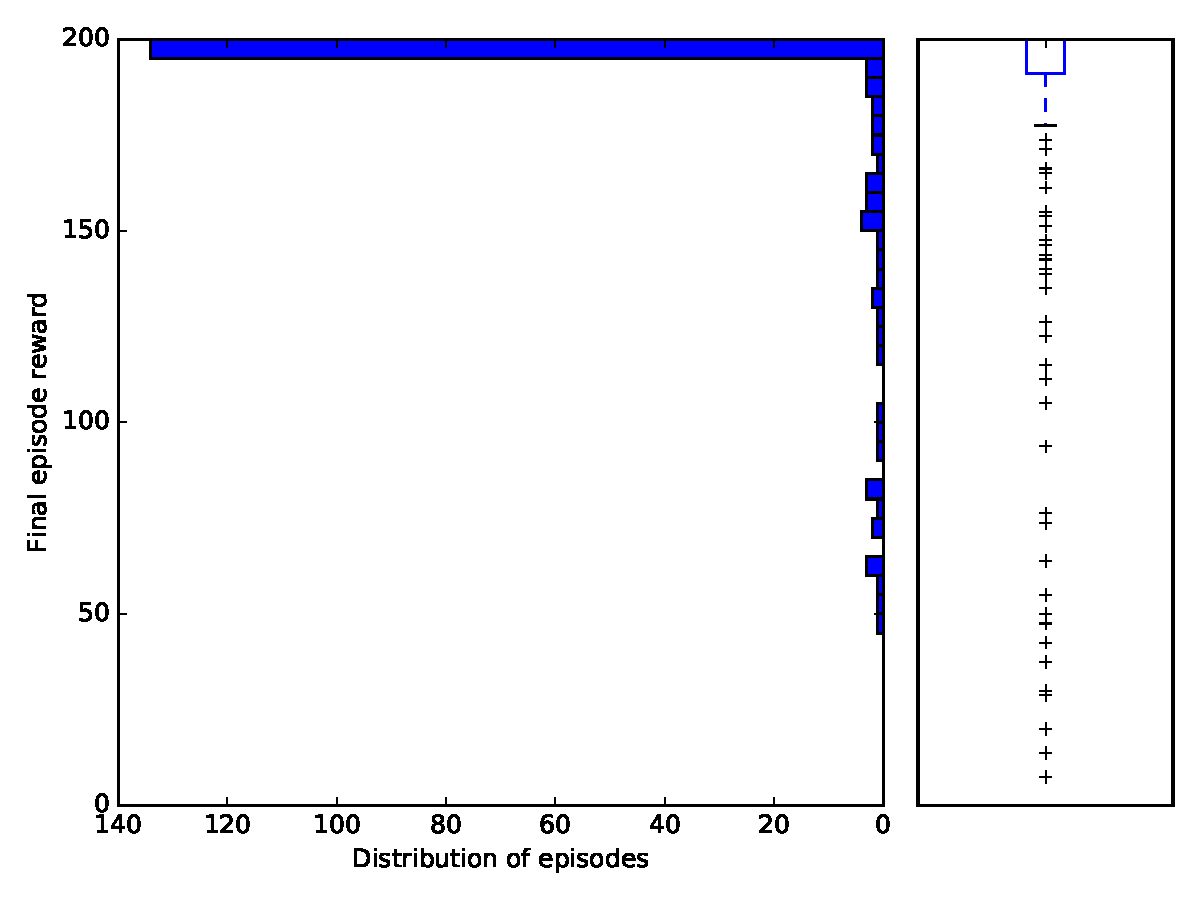
\includegraphics[width=0.49\linewidth]{fig/20perms_distrib_1ep.pdf}}
	\subfloat[][Trials of 2 episodes]{
		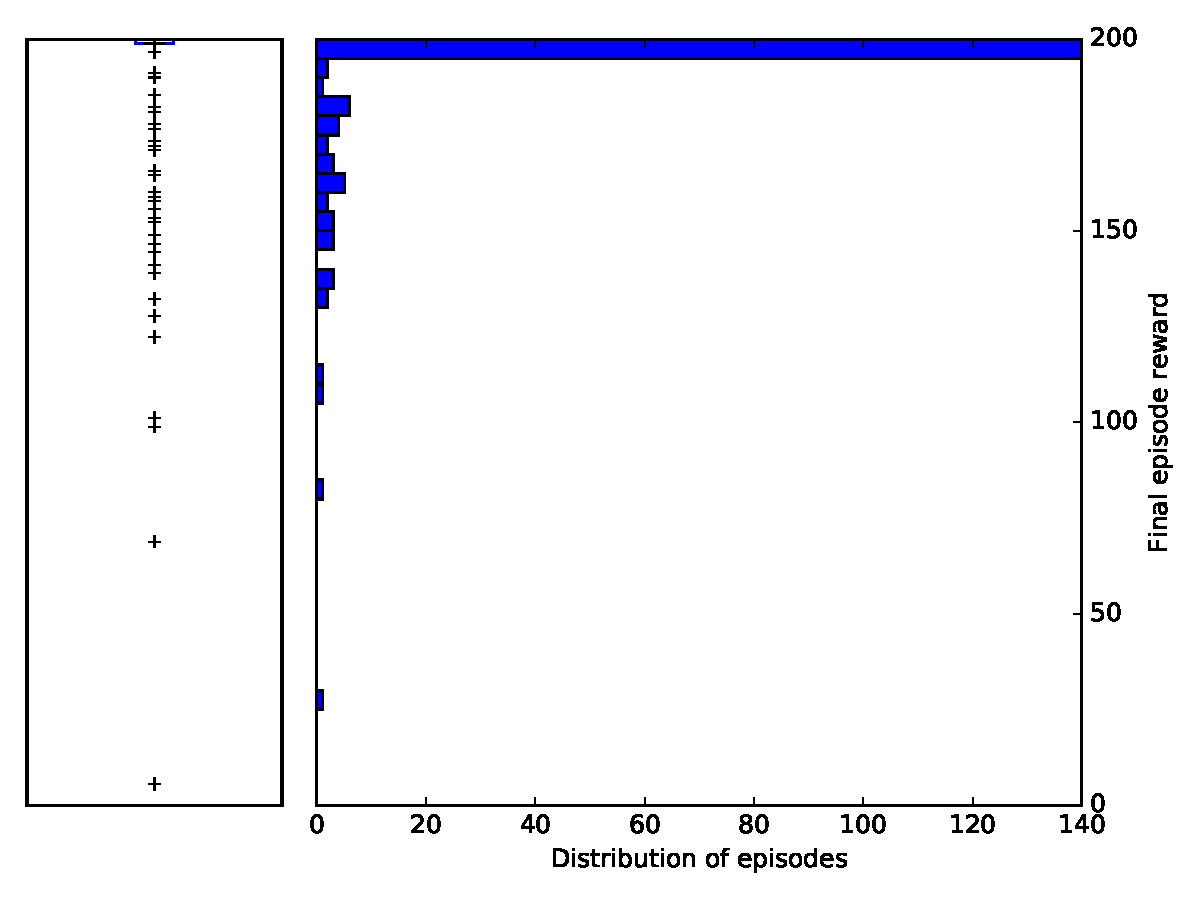
\includegraphics[width=0.49\linewidth]{fig/20perms_distrib_2ep.pdf}}
	\caption{Distributions of the total reward accumulated during the last
	episode of trials. 180 trials are played both in the case of
	single-episode trials and dual-episode trials. This shows the
	distribution of rewards obtained after playing 10 times each
	permutation of the \textbf{training} set. No action inversion is performed.}
	\label{fig:20perms_distrib}
\end{figure}

\begin{figure}[H]
	\centering
	\subfloat[][Trials of 1 episode]{
		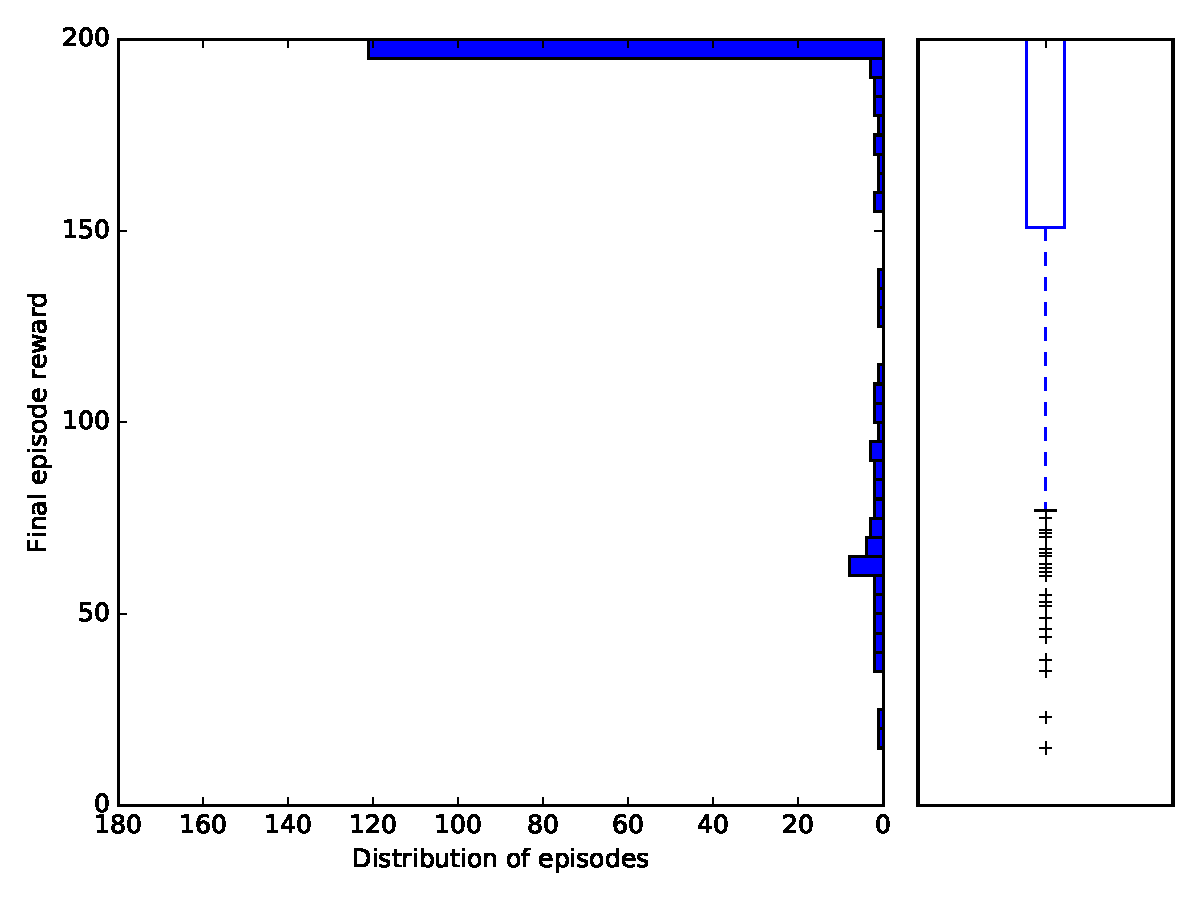
\includegraphics[width=0.49\linewidth]{fig/20perms_unseen_distrib_1ep.pdf}}
	\subfloat[][Trials of 2 episodes]{
		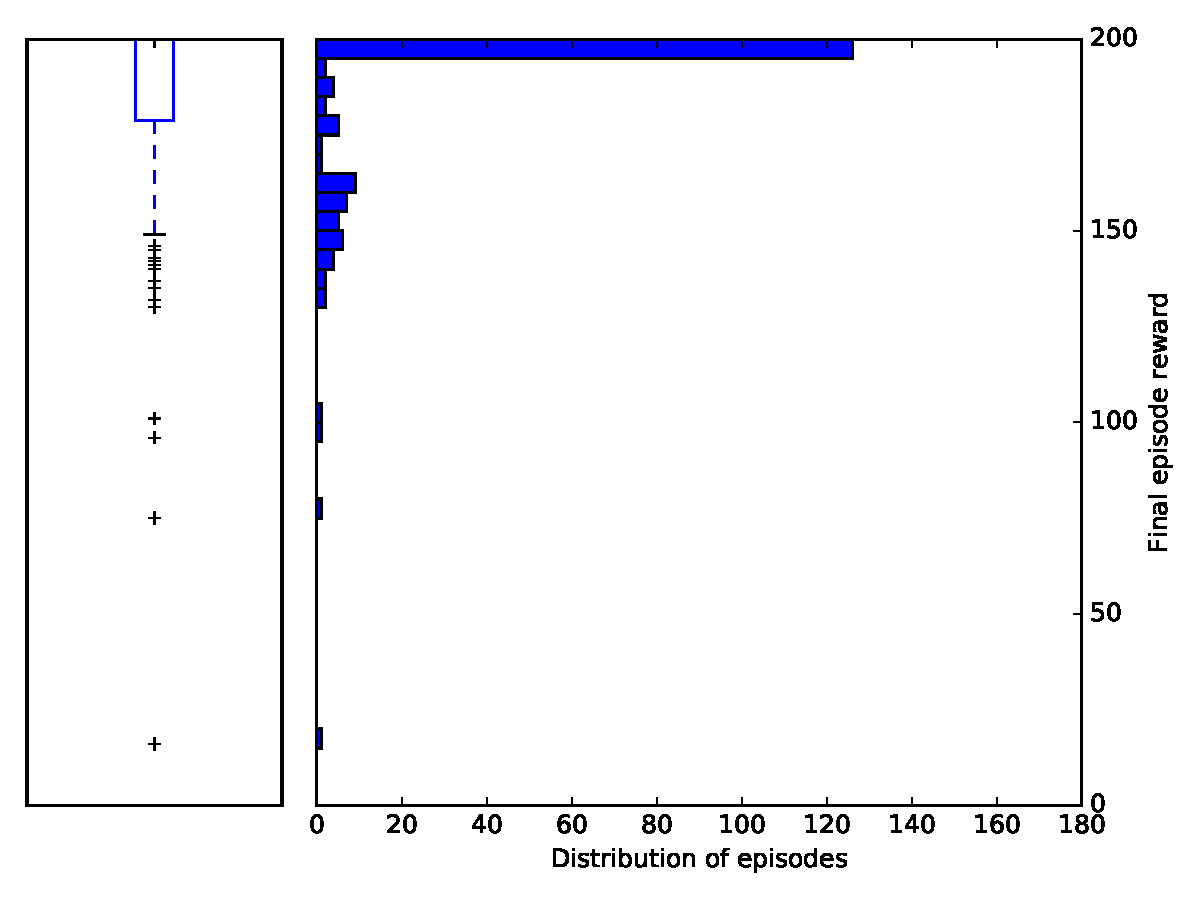
\includegraphics[width=0.49\linewidth]{fig/20perms_unseen_distrib_2ep.pdf}}
	\caption{Distributions of the total reward accumulated during the last
	episode of trials. This shows the distribution of rewards obtained
	after playing 30 times each permutation of the \textbf{test} set. No action
	inversion is performed.}
	\label{fig:20perms_unseen_distrib}
\end{figure}

To compare the two settings, we fix the agent's learnable parameters and make
it play 180 trials (resetting its hidden state before every trial). Every 
CartPole problem in the distribution is played the same amount of times.
Fixing the agent's learnable parameters means that we do not change
any of the weights of the neural network that represents the meta-learning
agent. We should perhaps emphasize that this means we do not train the agent
anymore; and that we expect the agent to learn \textbf{after training} still,
even though its weights are fixed.\\

Figure~\ref{fig:20perms_distrib} shows both a histogram and a boxplot describing
the final reward distributions in the single and dual episode situations. 
Although the difference is slight, and seeing that the number
of successes (a final reward of 195 or more, corresponding to the uppermost
bar) is almost exactly the same, there is definitely a difference in when the
failures occur. For the single episode setting, all failures are distributed
in a relatively uniform way spanning from 50 to 195; whereas they cluster 
slightly above 150 in the dual episode setting. The boxplots clearly show
a more compact distribution (and so a generally higher reward) in the dual
episode setting.\\

The agent seems to learn from the first episode to improve its performance in
the second. This is even clearer when we run the same experiment on unseen
permutations. As shown on Figure~\ref{fig:20perms_unseen_distrib}, where the
agent played every permutation of the test set for 30 trials, playing 180
trials in total to allow for comparison to the previous experiment, the agent
playing single-episode trials fails more often with a reward around 50. The
dual-episode setting shows again a capability to learn from the first episode
to improve performance in the second. We will later analyse performance
with longer trials containing more episodes.\\

Even more impressingly, if we add the inversion of the left and right actions
with a probability of 0.5 at the start of every trial, this effect is
tremendously magnified. For seen permutations
(Figure~\ref{fig:20permsLR_distrib}), there are about 40 more successes (out of
180) when playing two episodes than when playing only one; for unseen
permutations, this number climbs to about 70 out of 180. The single-episode
agent succeeds shy of 100 trials out of 180 where the dual-episode agent
comes close to 170 out of 180.\\

The reader might have noticed that the absolute performance for the agent
playing dual-episode trials is better when the problem is harder (with
inverted actions) as it succeeds close to 170 trials out of 180 whereas
for the simpler problem (without inverted actions), it only succeeds for
around 120 trials out of 180. We can only speculate as to why this result
occurs. We suggest this might be due to the fact that the harder problem
is impossible to be learned in one epiosde, thus forcing the agent to
really become a meta-learning agent, making it perform extremely well during
the second episode; whereas the simple problem might only be learned like
a standard reinforcement learning problem.\\

\begin{figure}
	\centering
	\subfloat[][Trials of 1 episode]{
		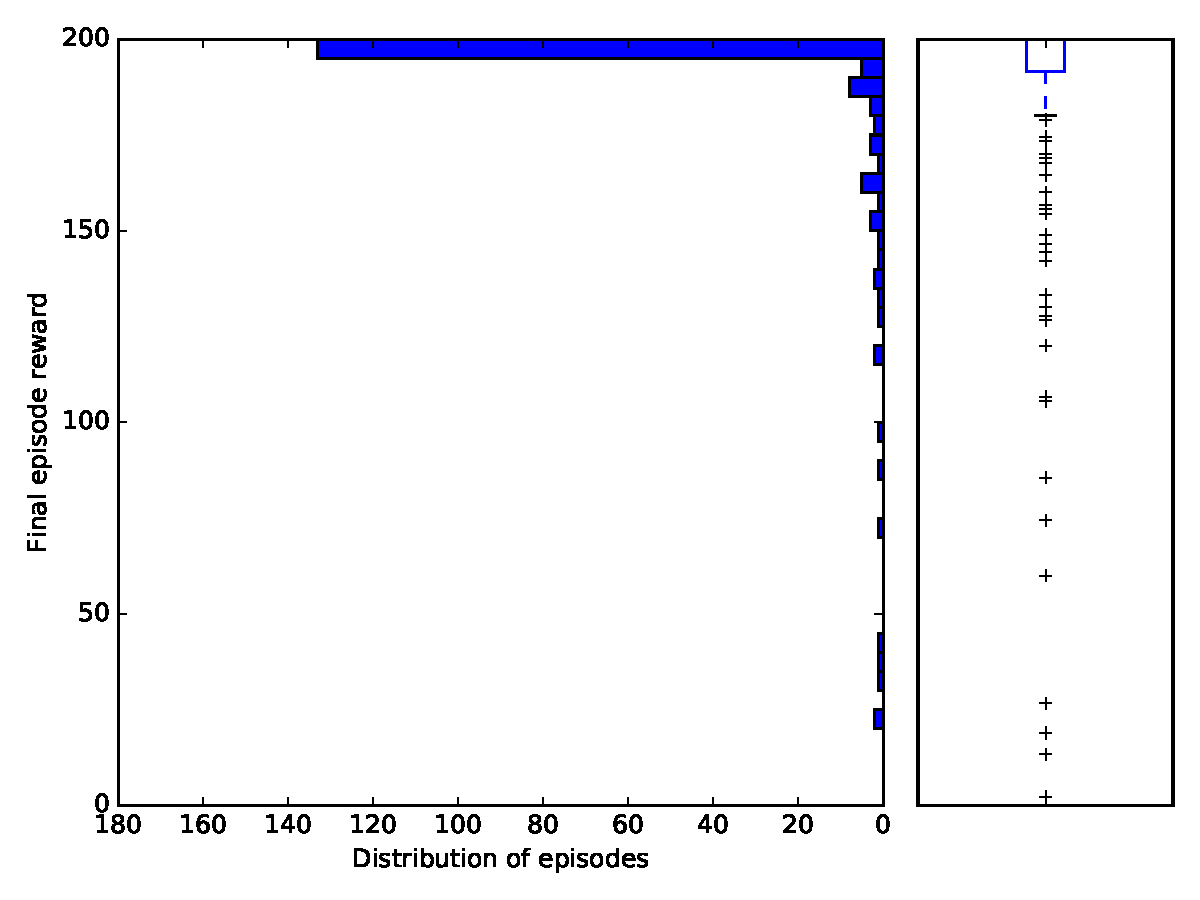
\includegraphics[width=0.49\linewidth]{fig/20permsLR_distrib_1ep.pdf}}
	\subfloat[][Trials of 2 episodes]{
		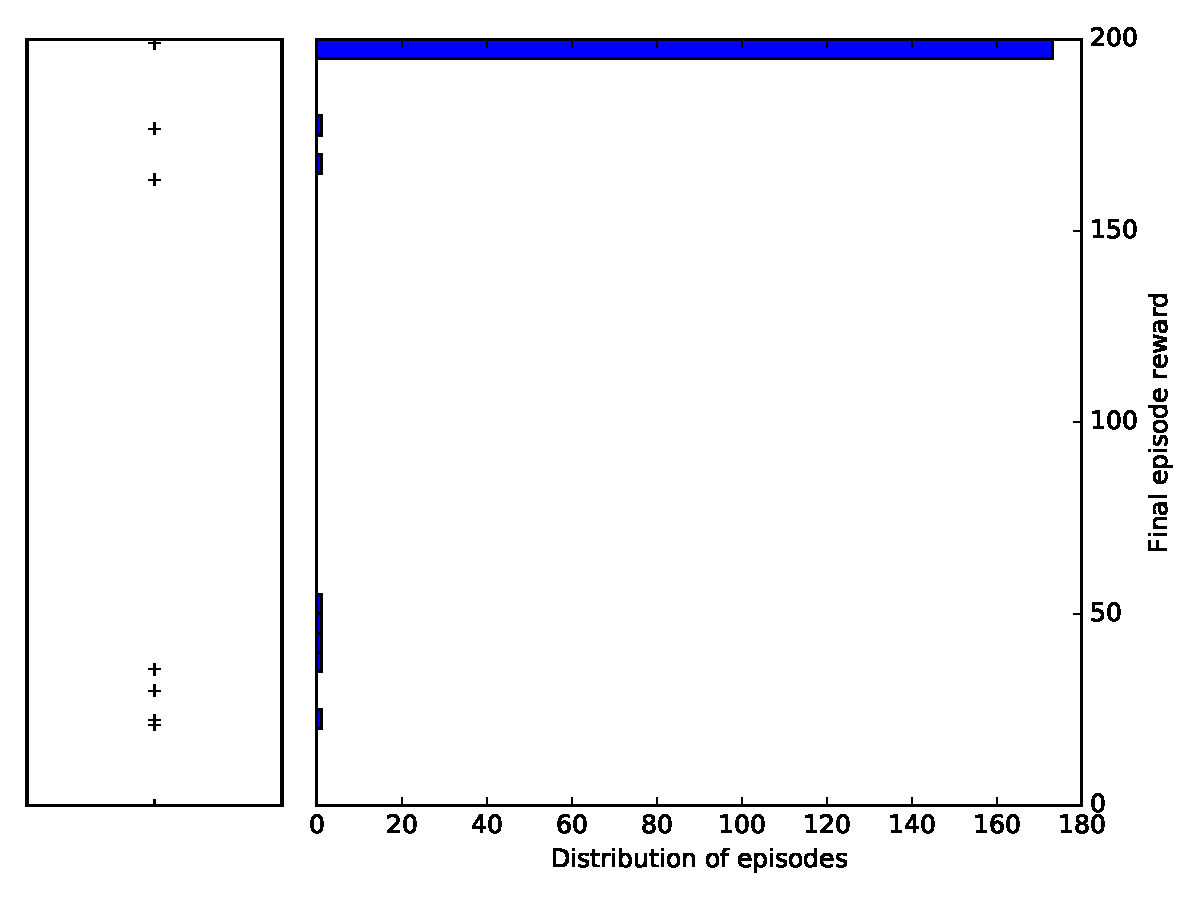
\includegraphics[width=0.49\linewidth]{fig/20permsLR_distrib_2ep.pdf}}
	\caption{Distributions of the total reward accumulated during the last
	episode of trials. This shows the distribution of rewards obtained after
	playing each permutation of the \textbf{training} set 5 times with action 
	inversion and 5 times without action inversion.}
	\label{fig:20permsLR_distrib}
\end{figure}

\begin{figure}
	\centering
	\subfloat[][Trials of 1 episode]{
		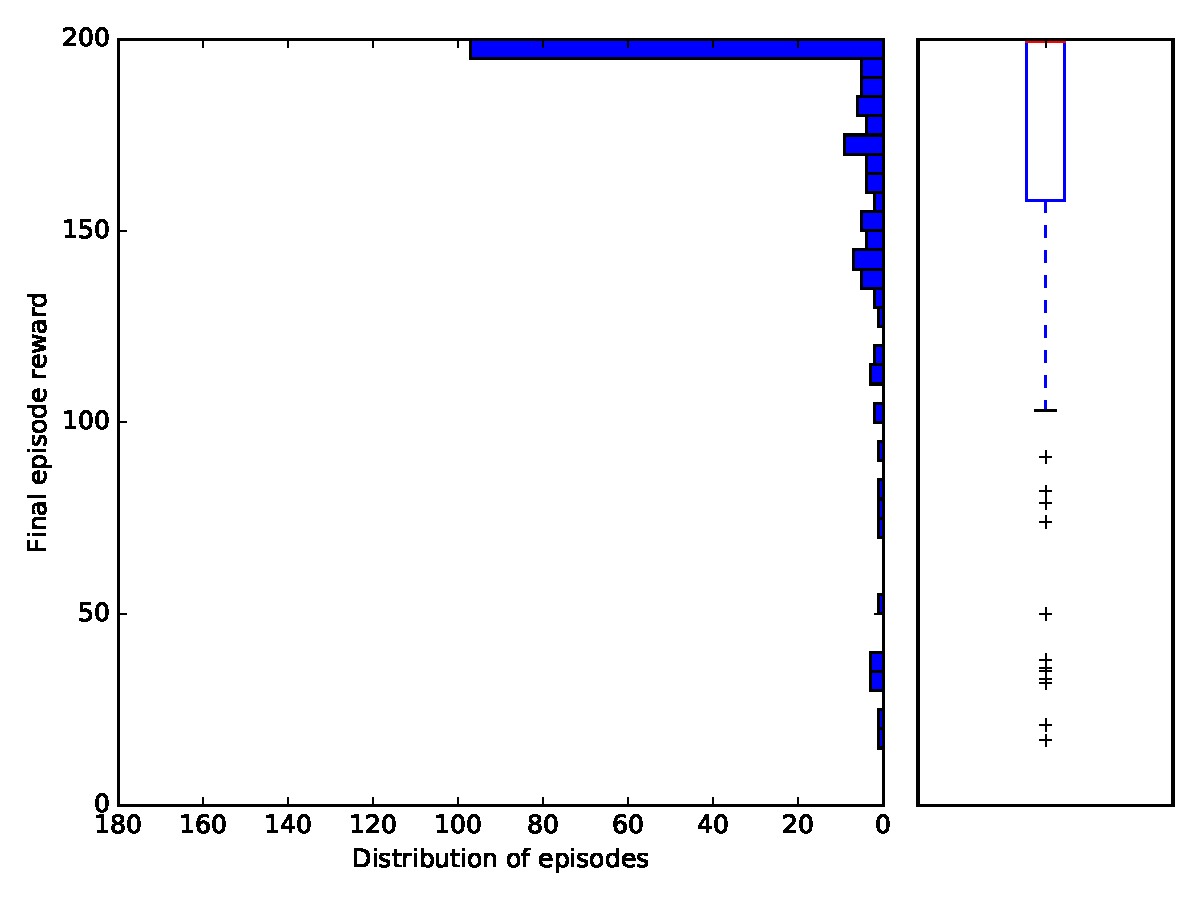
\includegraphics[width=0.49\linewidth]{fig/20permsLR_unseen_distrib_1ep.pdf}}
	\subfloat[][Trials of 2 episodes]{
		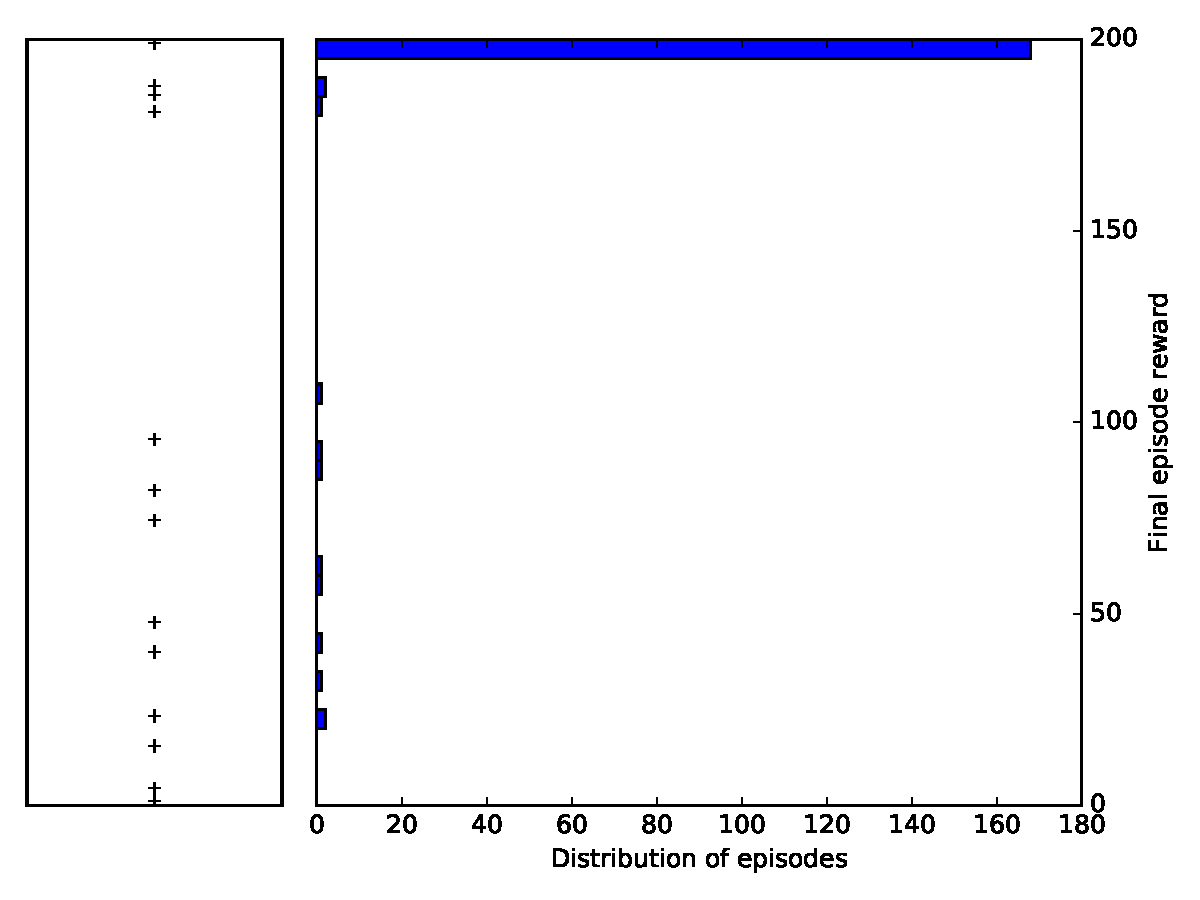
\includegraphics[width=0.49\linewidth]{fig/20permsLR_unseen_distrib_2ep.pdf}}
	\caption{Distributions of the total reward accumulated during the last
	episode of trials. This shows the distribution of rewards obtained after
	playing each permutation of the \textbf{test} set 5 times with action 
	inversion and 5 times without action inversion.}
	\label{fig:20permsLR_unseen_distrib}
\end{figure}

There are several surprises in these results. The first one is that a single
episode appears to be enough for an agent to discover how the observation has
been permutated in time to take action so that the pole stays balanced (at least
for a majority of trials), but playing a second episode improves the performance
of the agent (although at the cost of the reward of the first episode -- this
will be analysed in chapter~\ref{chap:reward_structure}).\\

The second one seems to be that in the setting of dual-episode trials, the
harder the problem is, the higher the number of successes will be. Indeed,
the performance of agents playing problems with inverted actions is 
significantly higher than the performance of agents playing problems without.


\subsubsection{Conclusion}
We have seen that applying meta-learning to a problem such as CartPole yields
interesting results on several aspects. The first one is that we can
indeed see information being passed from episode to episode to improve 
performance (in essence, learning is happening), but at the same some
behaviours deserve looking into:
\begin{itemize}
	\item the reward per episode seems to change quite a lot as a function
		of the number of episodes per trial and shows curious
		dynamics
	\item harder problems seem to make meta-learning more effective than
		simple problems; not only is the difference between 
		non-meta-learning and meta learning larger, but the absolute
		performance of the meta-learning agent on a harder problem
		is better than the absolute performance of the meta-learning
		agent on a simpler problem.
\end{itemize}

We will now look into more details as to why these behaviours occur.






\chapter{Issues with the reward structure}
\label{chap:reward_structure}
\begin{quotation}
\noindent ``\emph{quote}''
\begin{flushright}\textbf{author}\end{flushright}
\end{quotation}

Let us now look at why the reward of the first episode in a dual-episode
trial drops to random policy level when we know the agent is able to receive
an almost perfect reward in a single-episode trial. To understand why, we will
keep the same setting as previously \todo{ref to param table}.

\section{Training for more episodes}
There is a recurrent pattern visible in Figure~\ref{fig:20permsLR_training}.
Indeed, no matter the number of episodes in each trial, the last one will
always reach optimal or near-optimal performance while all previous episodes
will receive a reward which corresponds to following a random policy.
This is confirmed by the plots of Figure~\ref{fig:20permsLR_rewards} which
show the rewards obtained by playing several trials of 2, 5 and 10 episodes
(after having trained on trials of equal length) over all the permutations of
the training set. Only the last episode of the trial will succeed or almost
succeed.

\begin{figure}
	\centering
	\subfloat[][Training over 1 episode]{
		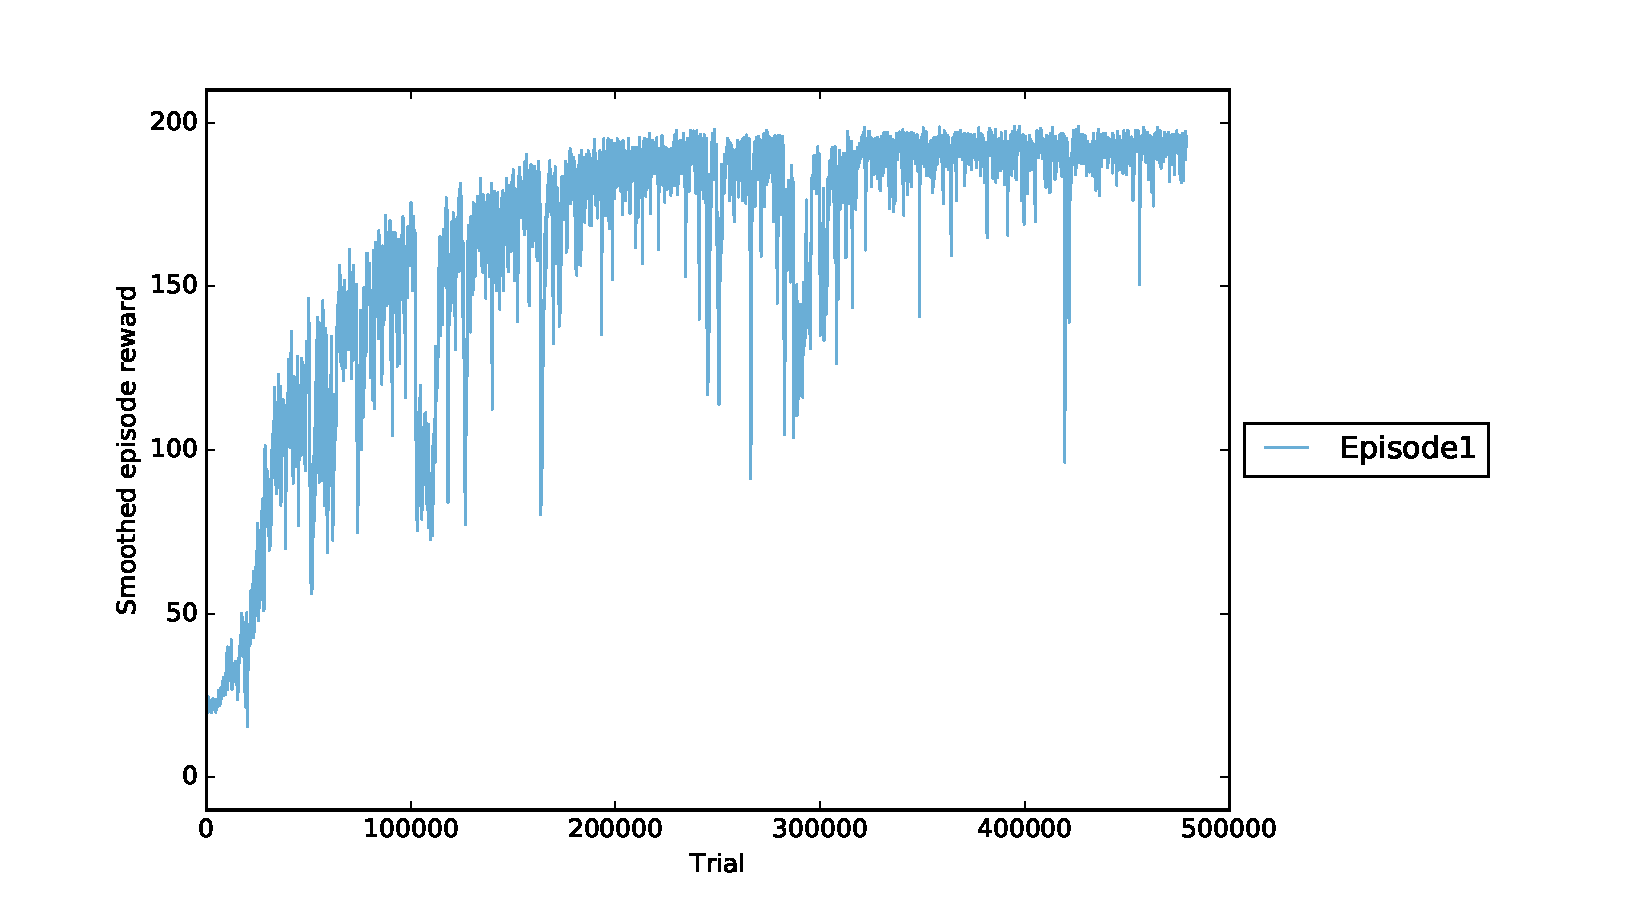
\includegraphics[width=0.49\linewidth]{fig/20permsLR1ep_training.pdf}}
	\subfloat[][Training over 2 episodes]{
		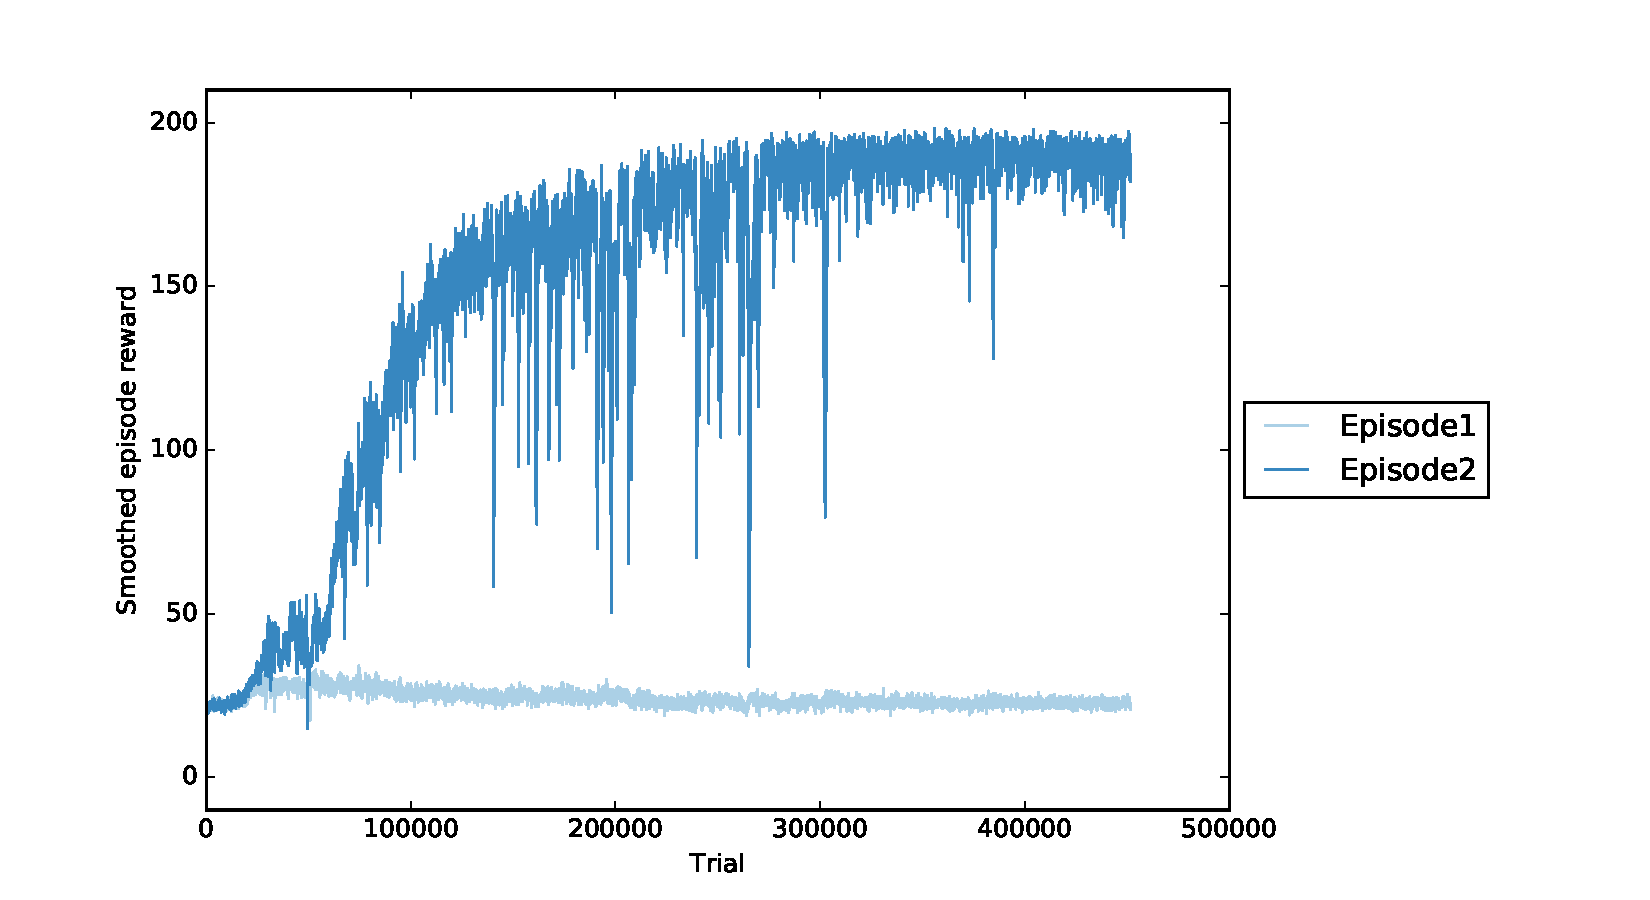
\includegraphics[width=0.49\linewidth]{fig/20permsLR2ep_training.pdf}}
	\\
	\subfloat[][Training over 3 episodes]{
		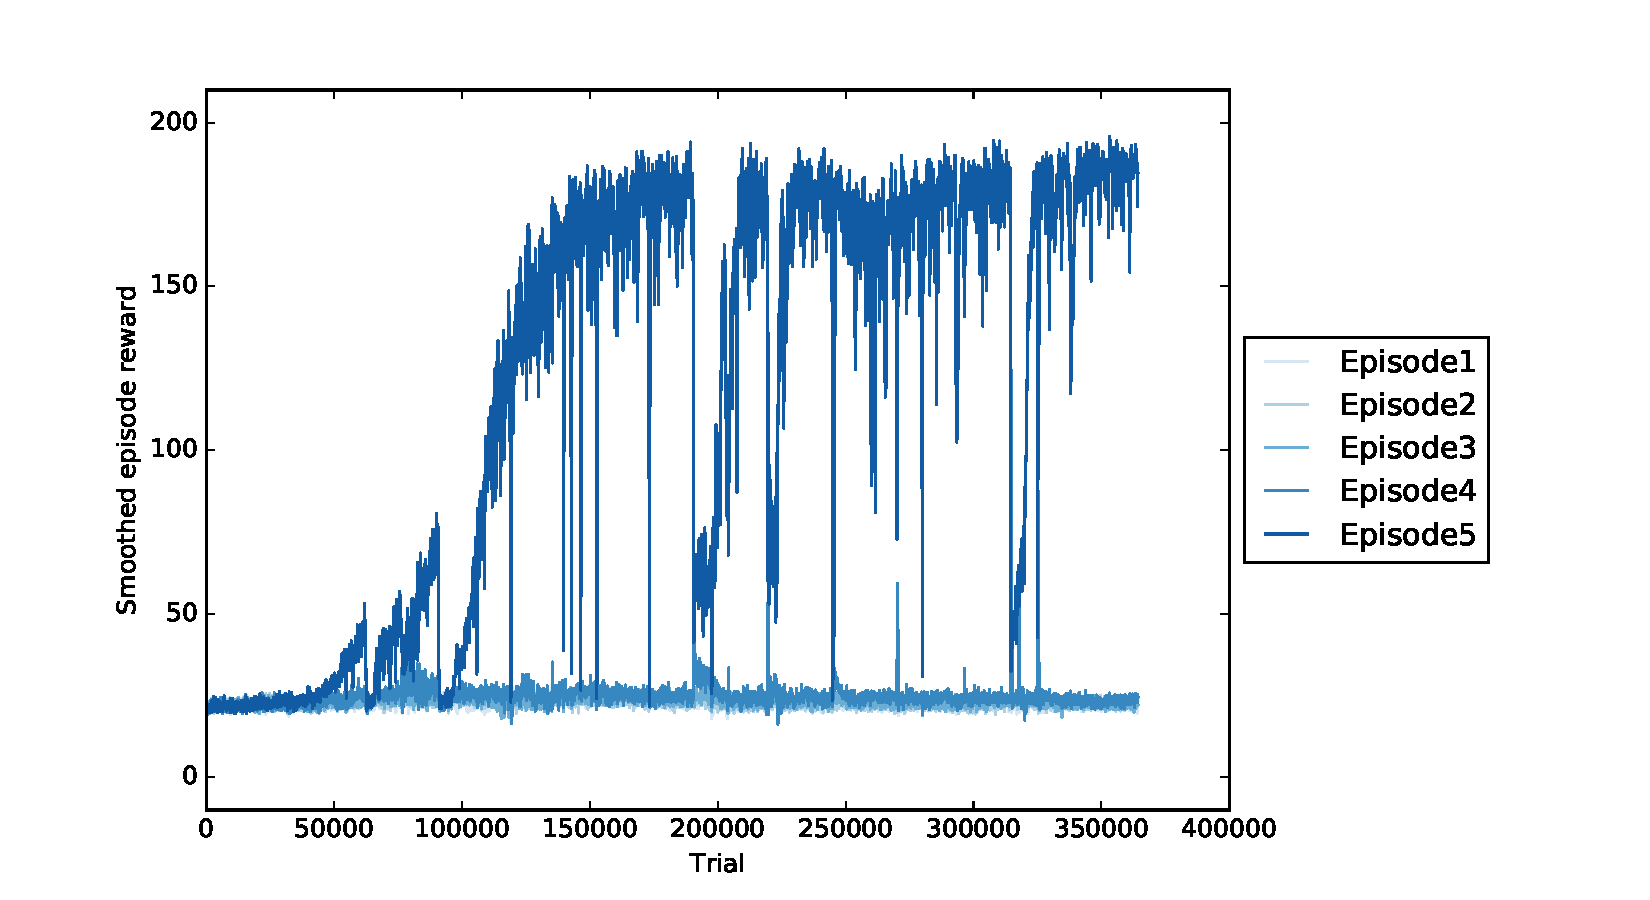
\includegraphics[width=0.9\linewidth]{fig/20permsLR5ep_training.pdf}}
	\caption{}
	\label{fig:20permsLR_training}
\end{figure}

\begin{figure}
	\centering
	\subfloat[][2 episodes]{
		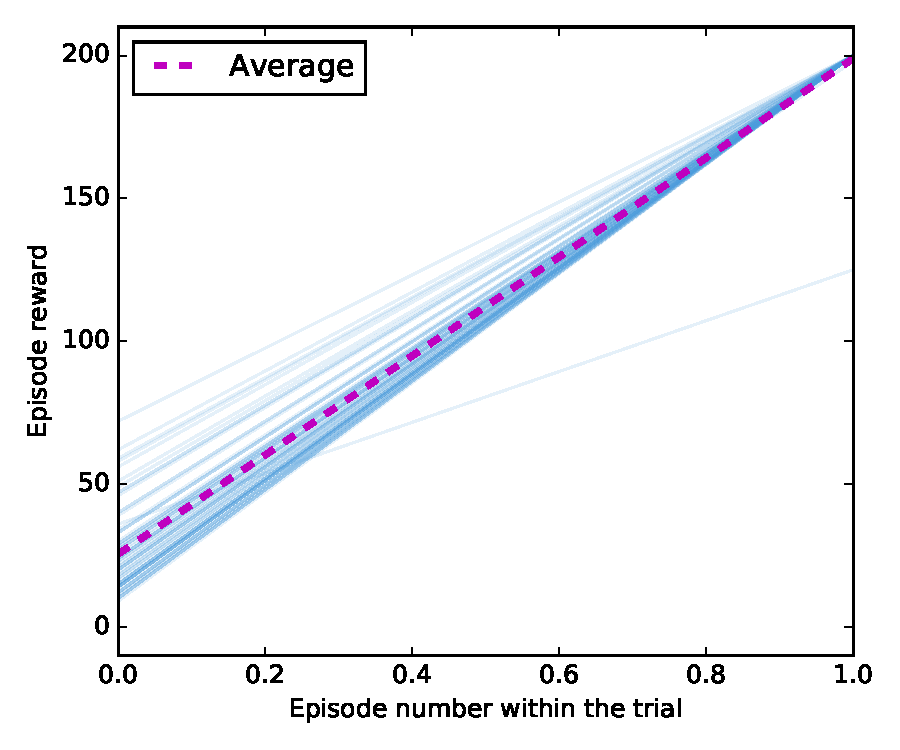
\includegraphics[width=0.33\linewidth]{fig/20permsLR2ep_rewards.pdf}}
	\subfloat[][5 episodes]{
		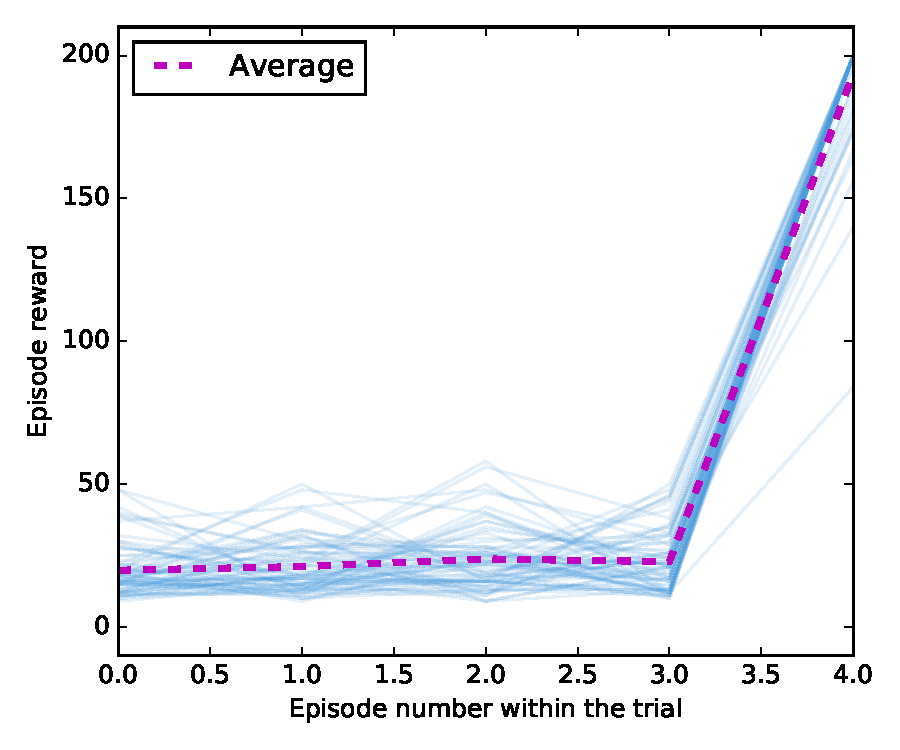
\includegraphics[width=0.33\linewidth]{fig/20permsLR5ep_rewards.pdf}}
	\subfloat[][10 episodes]{
		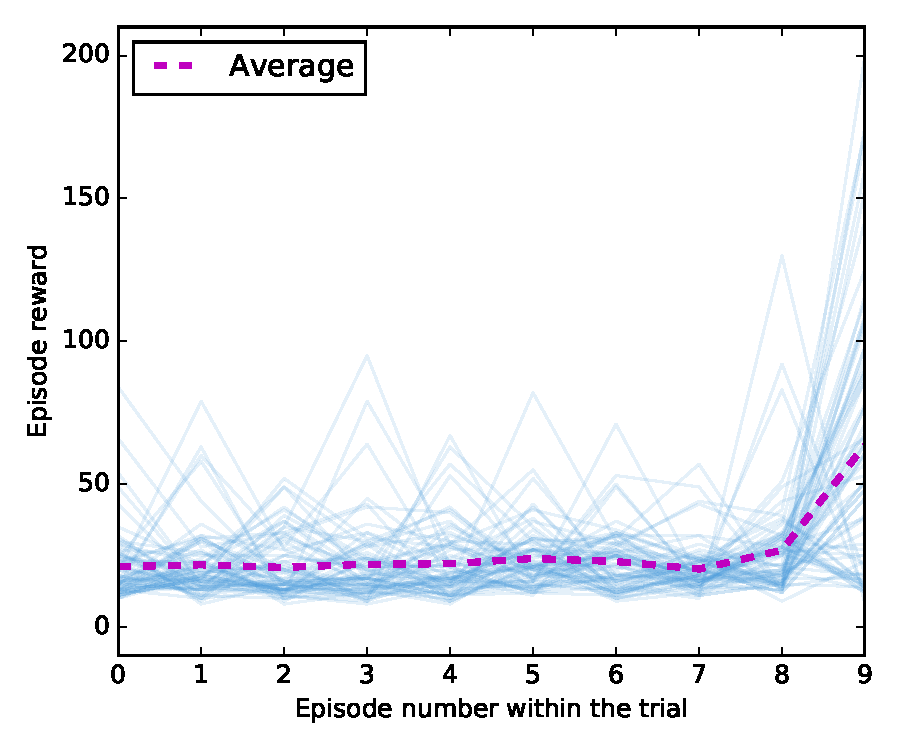
\includegraphics[width=0.33\linewidth]{fig/20permsLR10ep_rewards.pdf}}
	\caption{}
	\label{fig:20permsLR_rewards}
\end{figure}

\begin{figure}
	\centering
	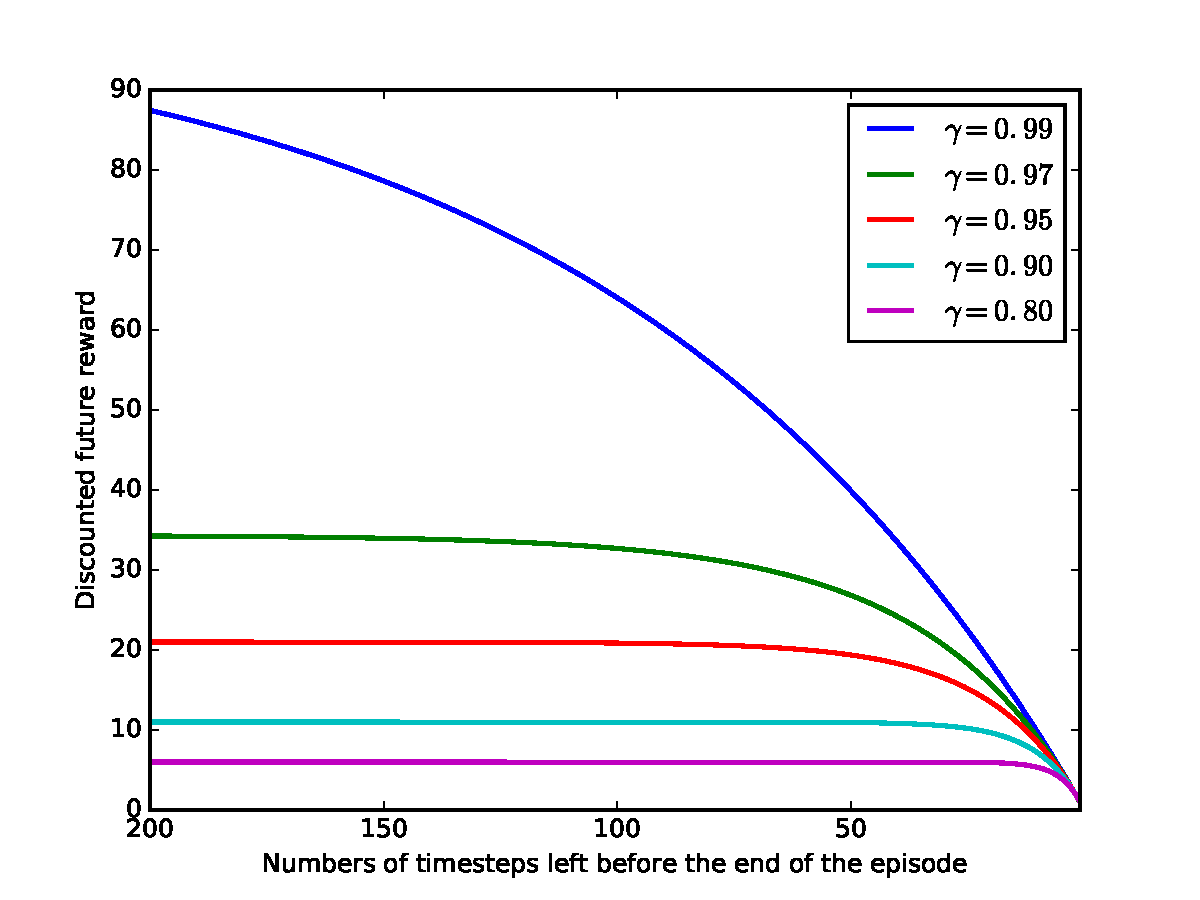
\includegraphics[width=0.8\linewidth]{fig/gamma_impact.pdf}
	\caption{}
	\label{fig:gamma_impact}
\end{figure}

\section{Problems with a 1-per-timestep reward}
This behaviour is linked to the dynamics of the expected future reward, 
the chosen discount factor and the reward structure of the environment.
In our case, the environment gives a constant +1 reward at every timestep of
an CartPole episode. If we choose a discount factor $\gamma=0.9$, the
discounted future reward at timesteps which are more than 50 timesteps away
from the end of the episode will be almost exactly equal (see 
Figure~\ref{fig:gamma_impact}).\\

This means that if an action that defines whether the episode ends or continues
at time $t$ has to be taken before time $t-50$, there is no way to link the
end of the episode with the action that was wrongly taken. This can be turned
around to say that actions do not really matter as long as the end of the
constant reward stream is more than 50 timesteps away for $\gamma=0.9$. 

\todo{why episode longer than 200 works?}


\section{Tuning discount factor}
Show different gammas

\begin{figure}
	\centering
	\subfloat[][$\gamma=0.82$]{
		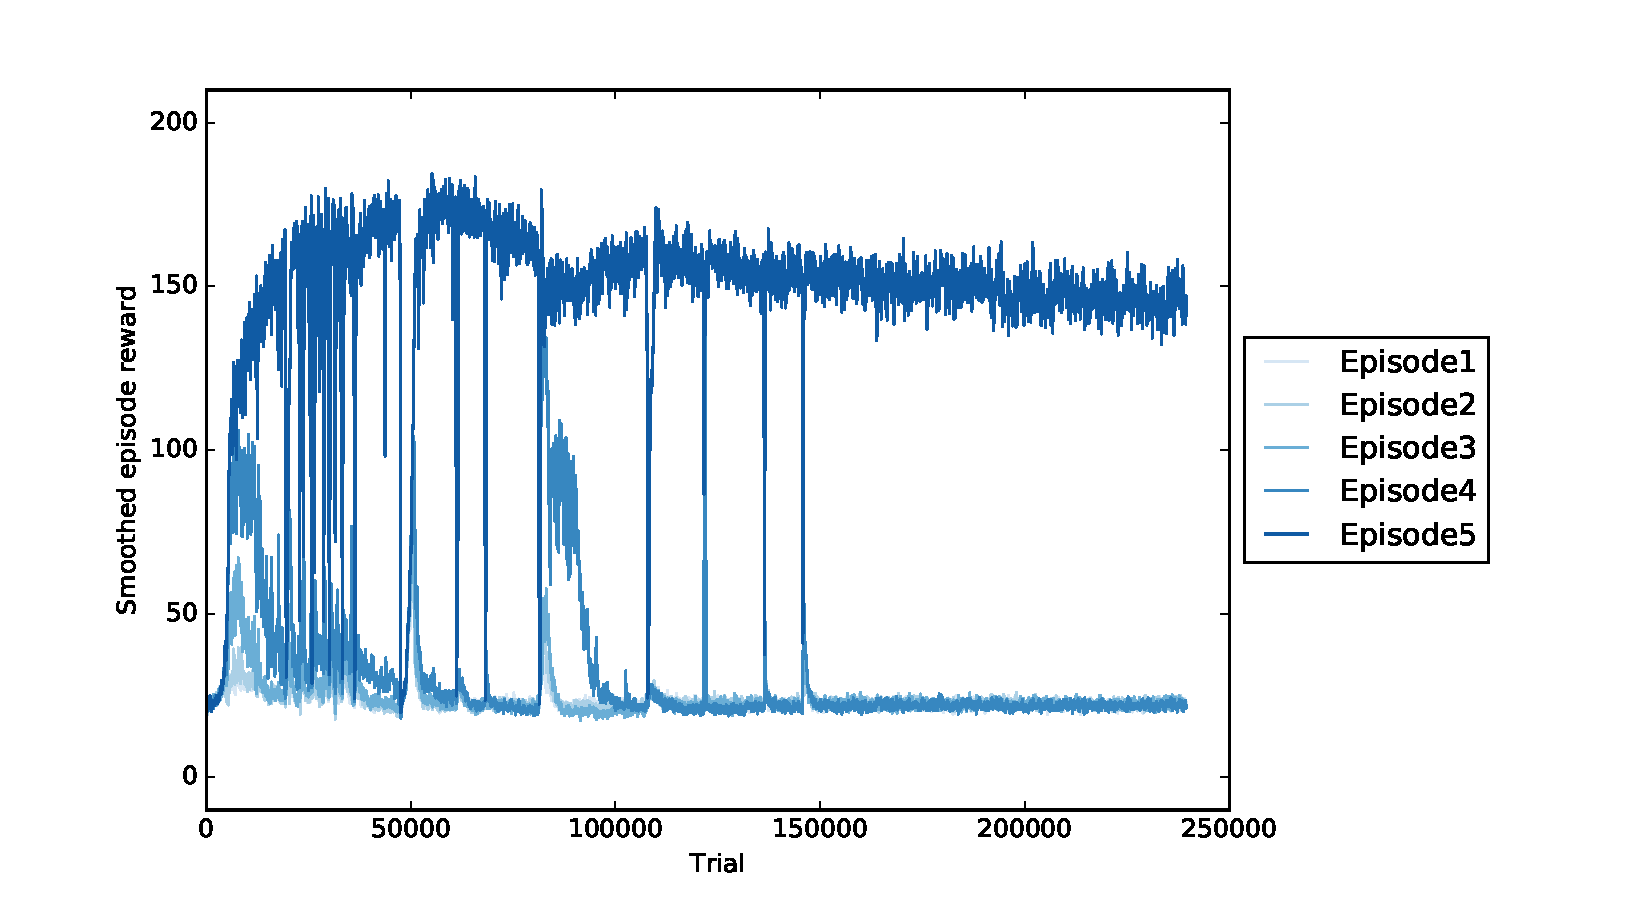
\includegraphics[width=0.49\linewidth]{fig/res_perms5ep_82.pdf}}
	\subfloat[][$\gamma=0.85$]{
		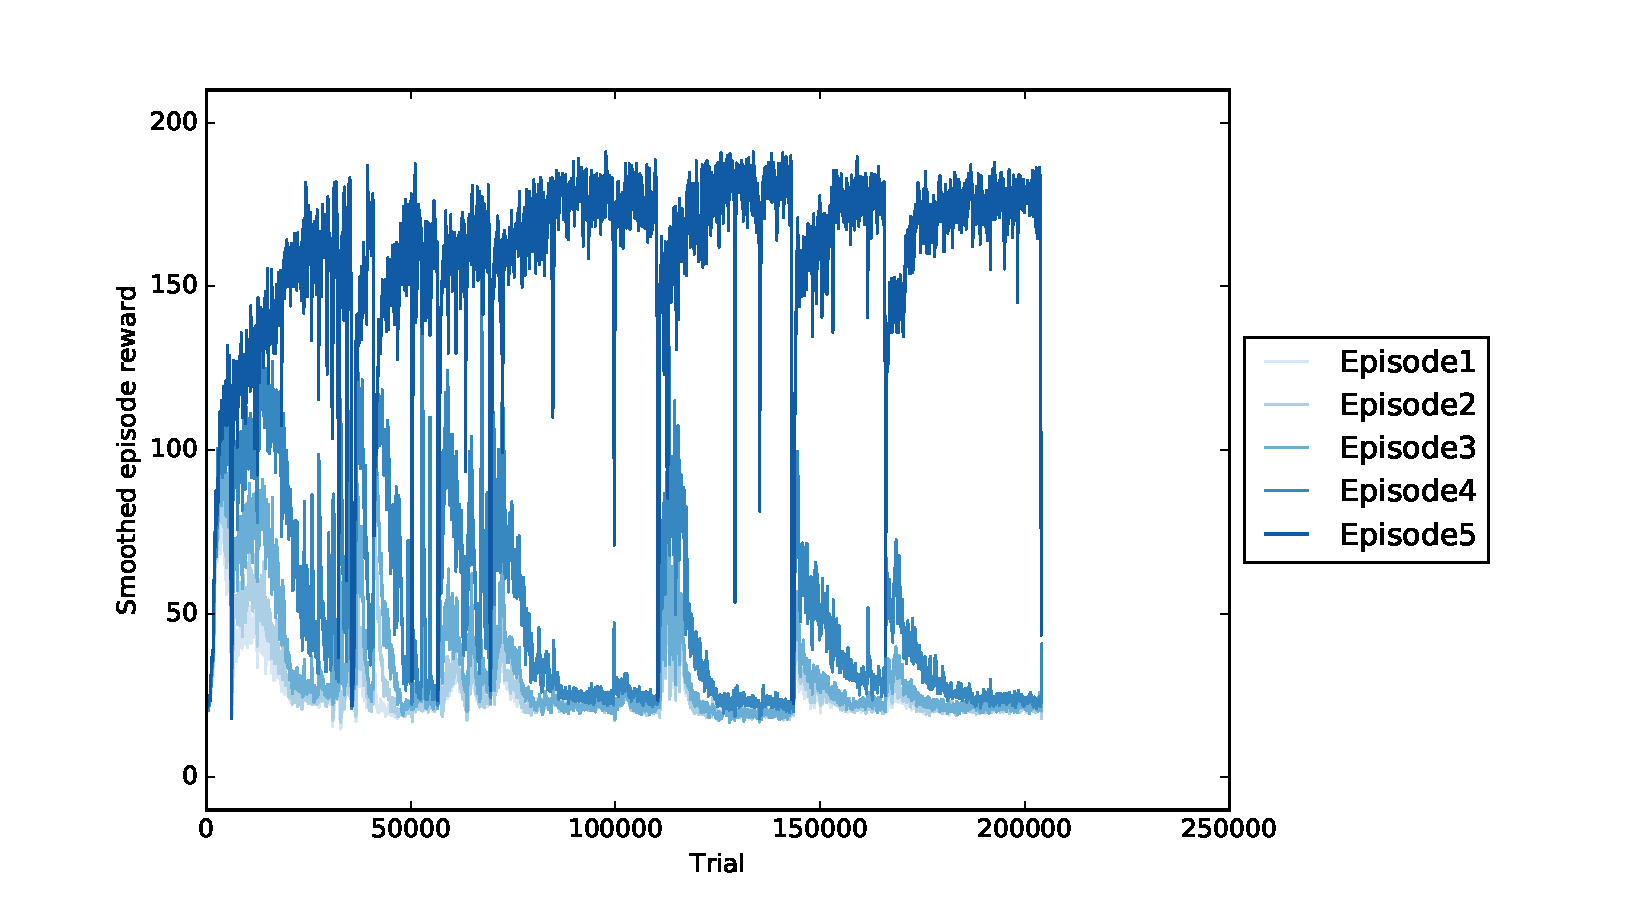
\includegraphics[width=0.49\linewidth]{fig/res_perms5ep_85.pdf}}
	\\
	\subfloat[][$\gamma=0.88$]{
		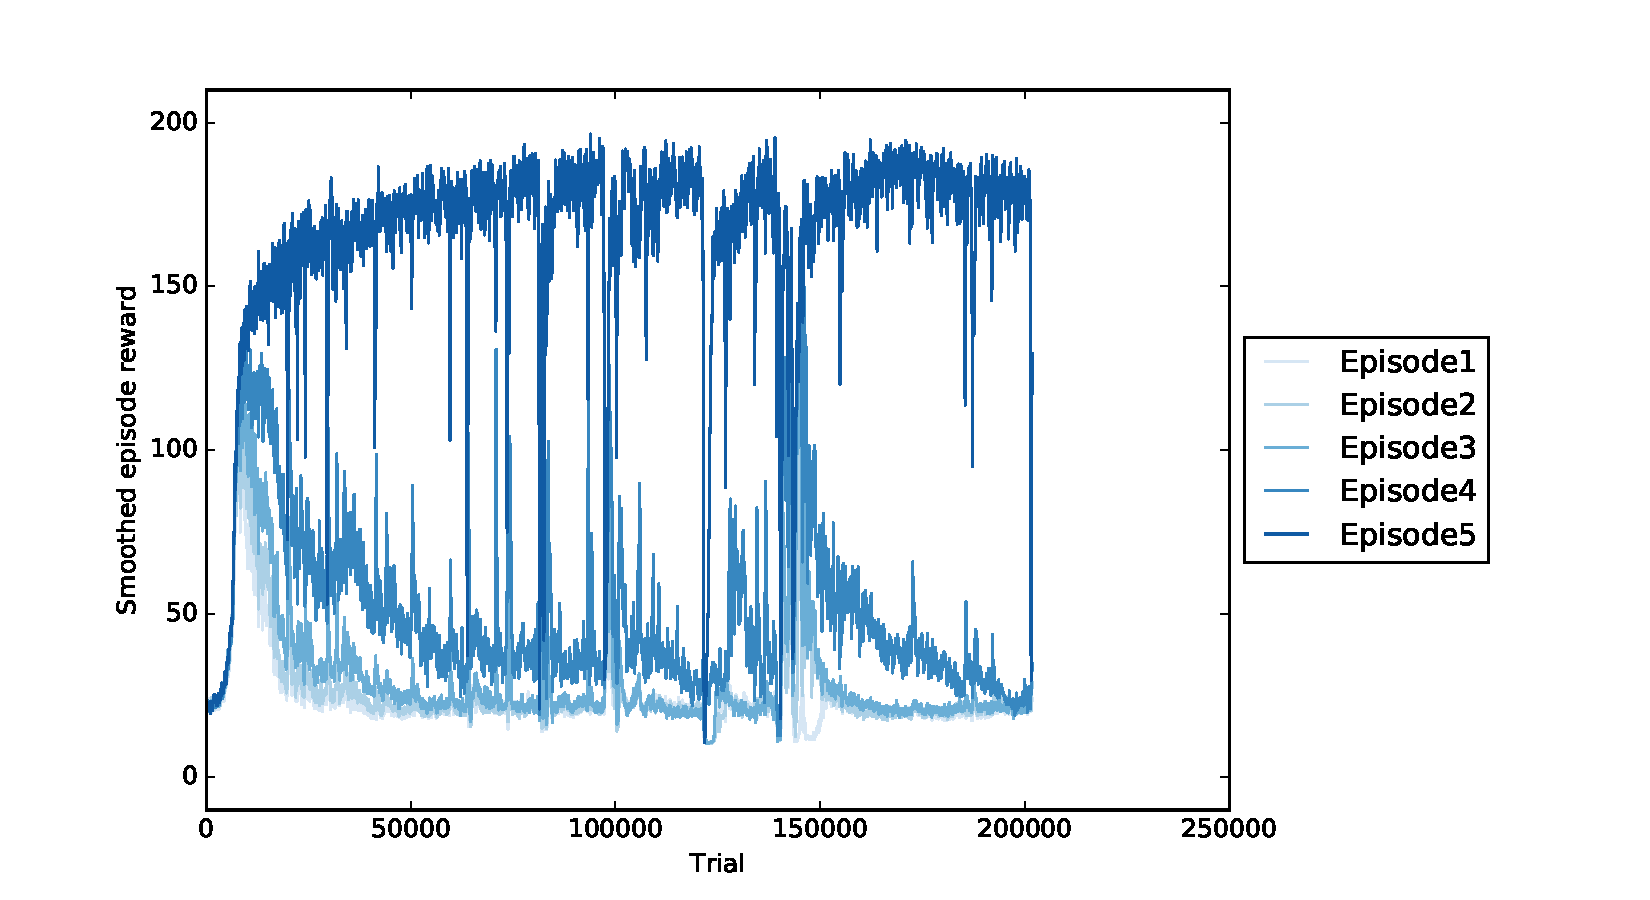
\includegraphics[width=0.49\linewidth]{fig/res_perms5ep_88.pdf}}
	\subfloat[][$\gamma=0.91$]{
		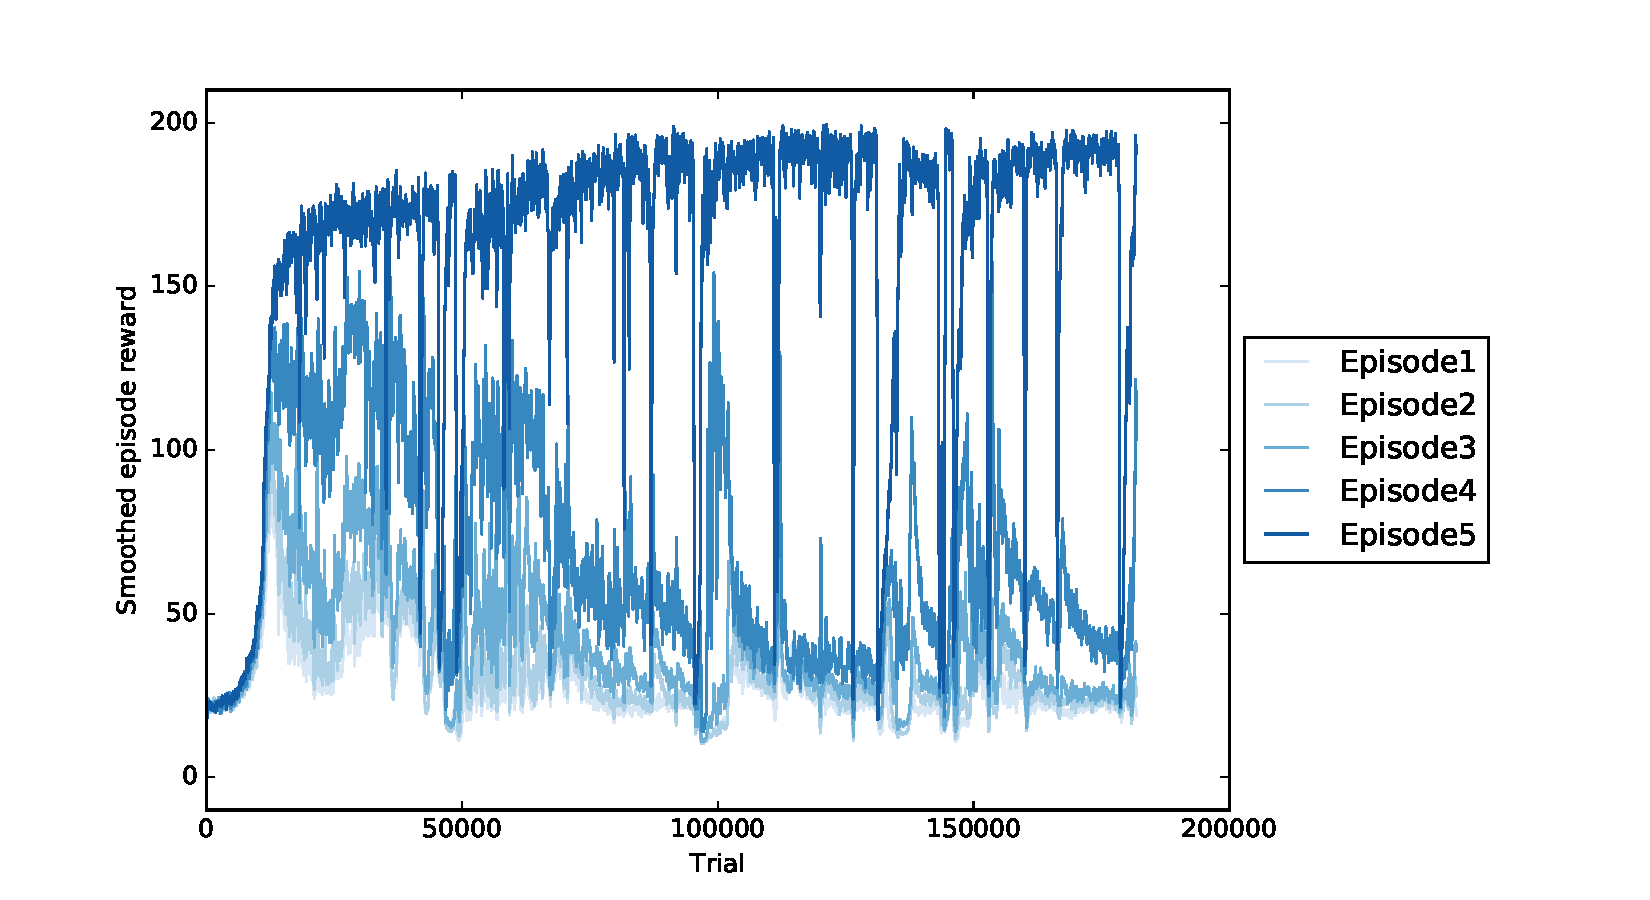
\includegraphics[width=0.49\linewidth]{fig/res_perms5ep_91.pdf}}
	\\
	\subfloat[][$\gamma=0.94$]{
		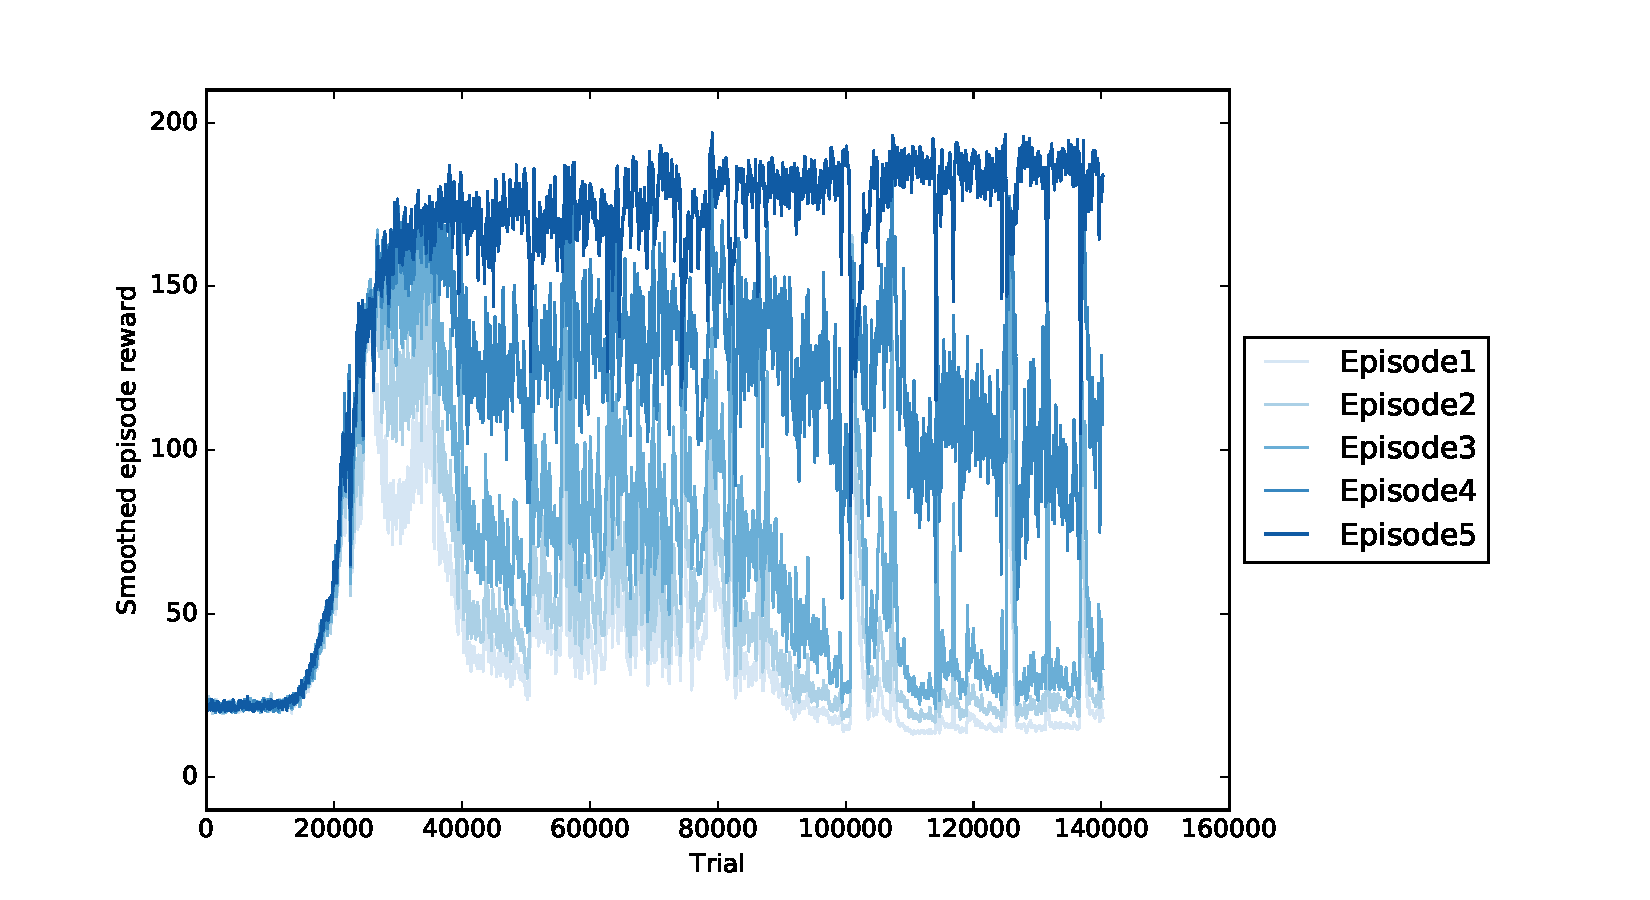
\includegraphics[width=0.49\linewidth]{fig/res_perms5ep_94.pdf}}
	\subfloat[][$\gamma=0.97$]{
		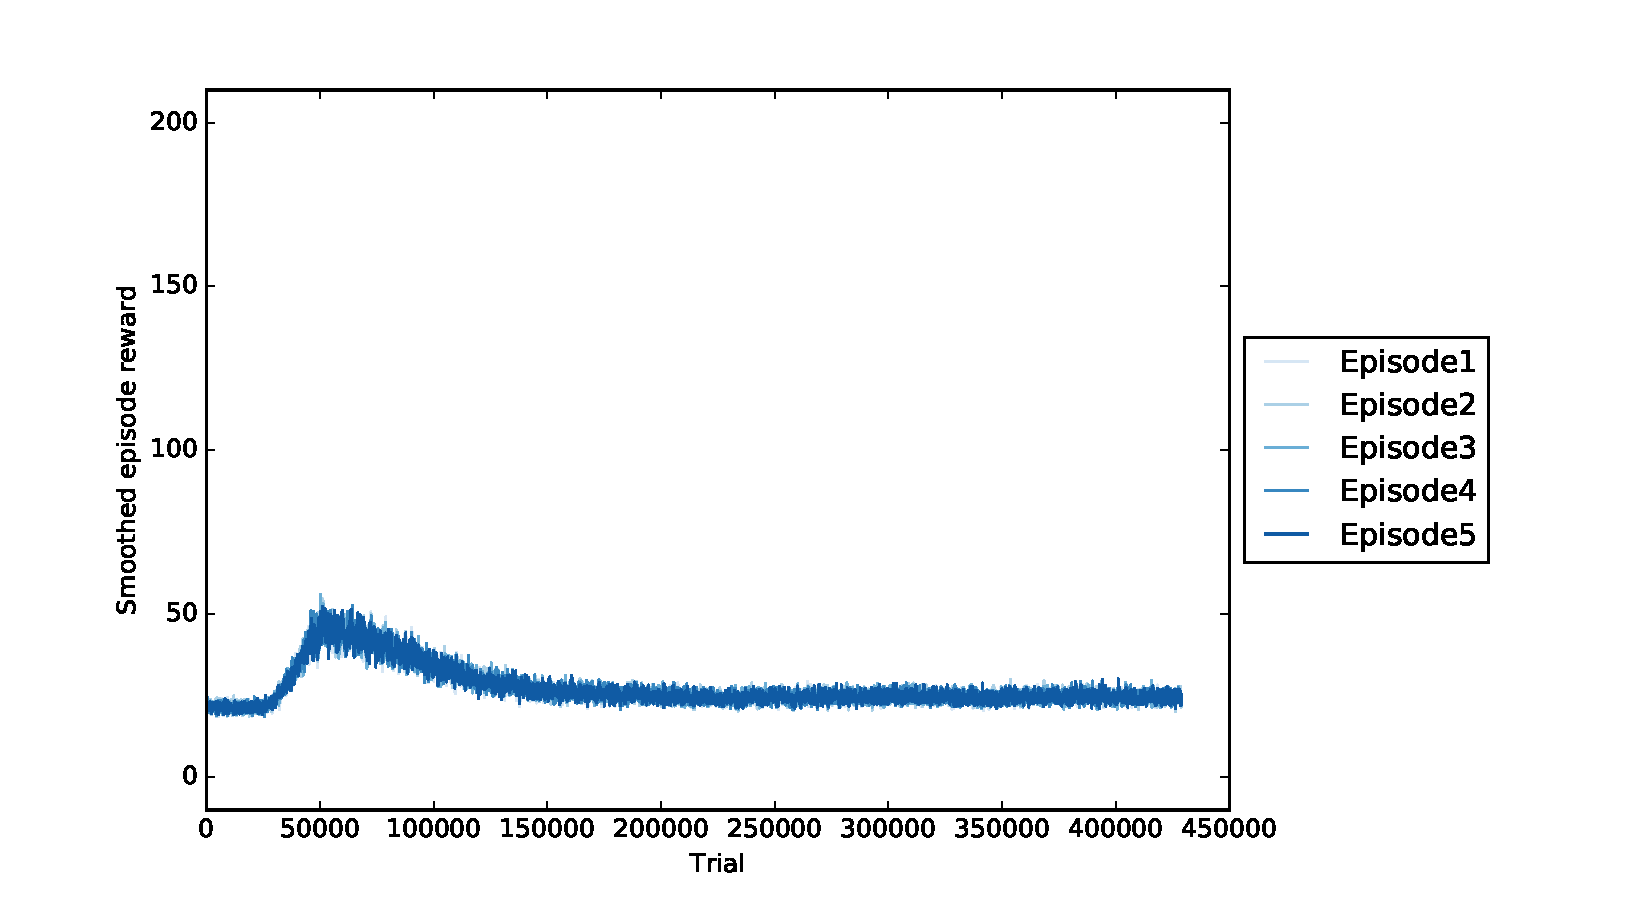
\includegraphics[width=0.49\linewidth]{fig/res_perms5ep_97.pdf}}
	\\
	\caption{}
	\label{fig:varied_gamma}
\end{figure}



\chapter{Injecting an informational reward}
\begin{quotation}
\noindent ``\emph{The ideal of behaviourism is to eliminate coercion: to apply
	controls by changing the environment in such a way as to reinforce the
	kind of behaviour that benefits everyone.}''
\begin{flushright}\textbf{Burrhus Frederic Skinner}\end{flushright}
\end{quotation}
\vspace*{0.5cm}


We have described in section \ref{section:problems_1_timestep_reward} why
a 1-per-timestep reward structure led to an undesired behaviour of laziness,
in which the agent only maximised its reward on the last episode of its
training trials.\\

We introduce a simple, yet effective way to allow problems with similar 
reward structures to be meta-learned. In hand-designed strategies aimed to
solve such problems, the designer holds the implicit knowledge that a short
episode is a bad thing, and treats the reward streams of each episode 
separately. In meta-learning, just like we feed back a termination flag, which
is not an environment-level value but rather a "process-level" value (where
the process is the training process we replicate in a trial); we can
introduce a process-level reward to give information to the agent 
performing the trial.\\

We propose to add a small negative reward at the end of each episode, 
interrupting the continuous reward stream to force the agent to perform
well for each of the episodes in the trial.\\

Our agent is trained on the training set of 18 permutations listed on table
\ref{tab:20perms}, on trials of 3 episodes. The reward for the last 
timestep of each episode is set to -10. Figure \ref{fig:magic} shows how
the episode-wise reward curve evolves during training. We see that all
three episodes reach a high reward, but more importantly, performance
increases for the second and third episode. \\

This is clearer on Figure~\ref{fig:magic_rewards}, where we see
that episodes 2 and 3 get a higher average than episode 1. We also see
however that letting the agent play beyond its training horizon leads to
a generally lower average reward. A second surprise is the fact that the
average reward for the third episode when testing on unseen permutations is
below the average reward of second episodes. It is however still above the average
reward for first episodes. We suspect this variance in the results is due
to the closeness in performance of all three episodes.\\

\begin{figure}
	\centering
	\subfloat[][Full training graph]{
		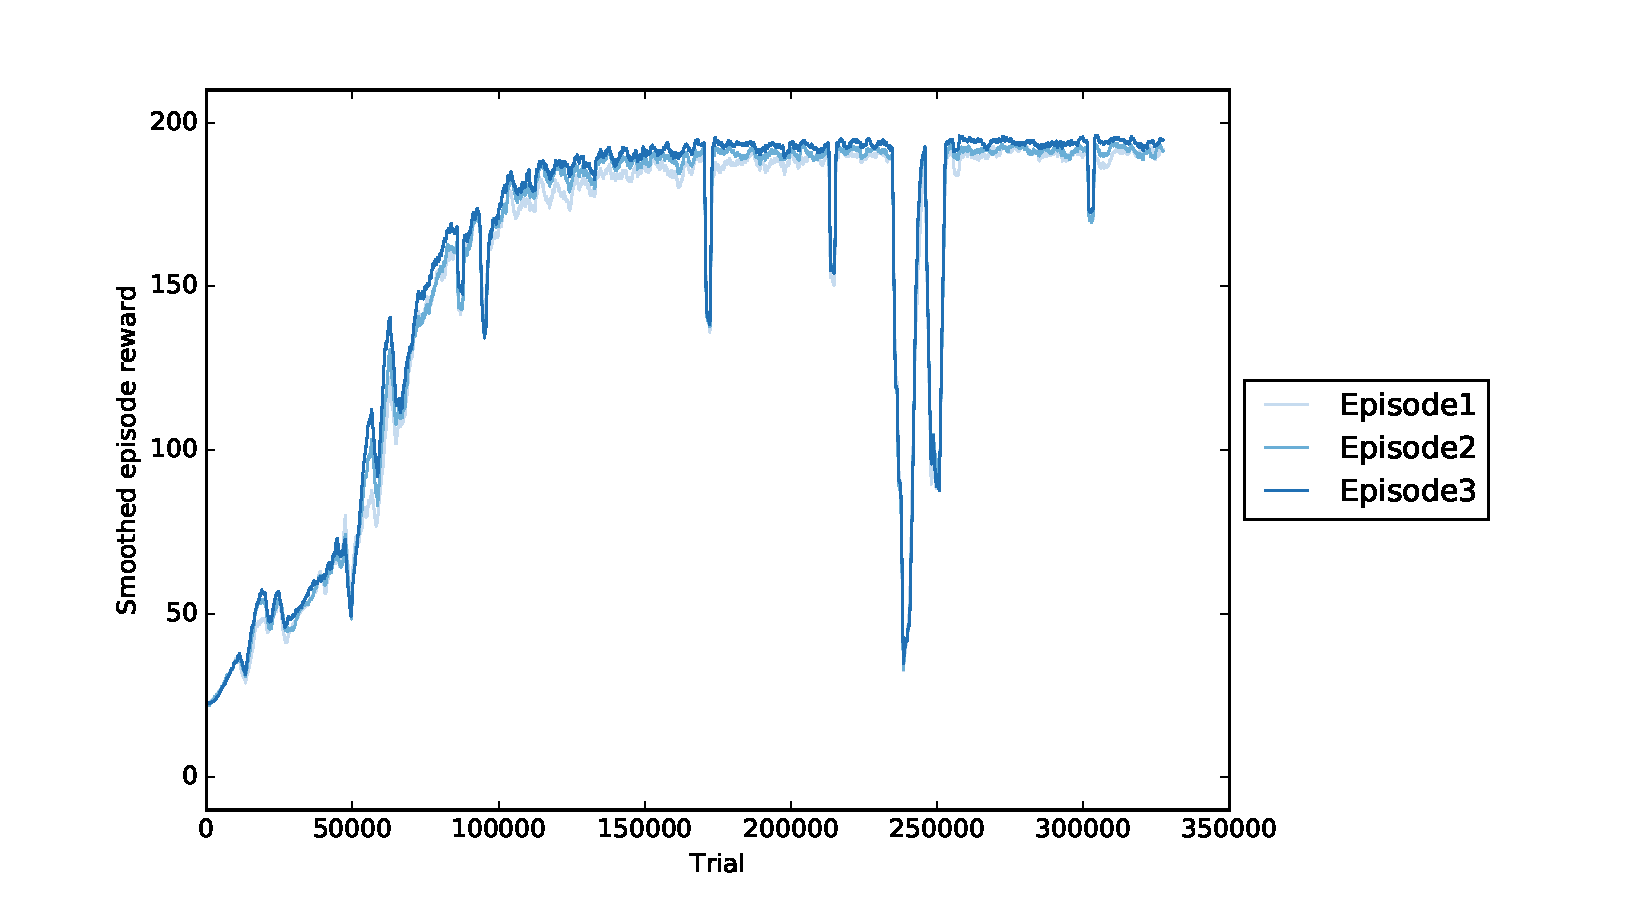
\includegraphics[width=0.8\linewidth]{fig/res_magic_neg10.pdf}}\\
	\subfloat[][Close-up of the last trials]{
		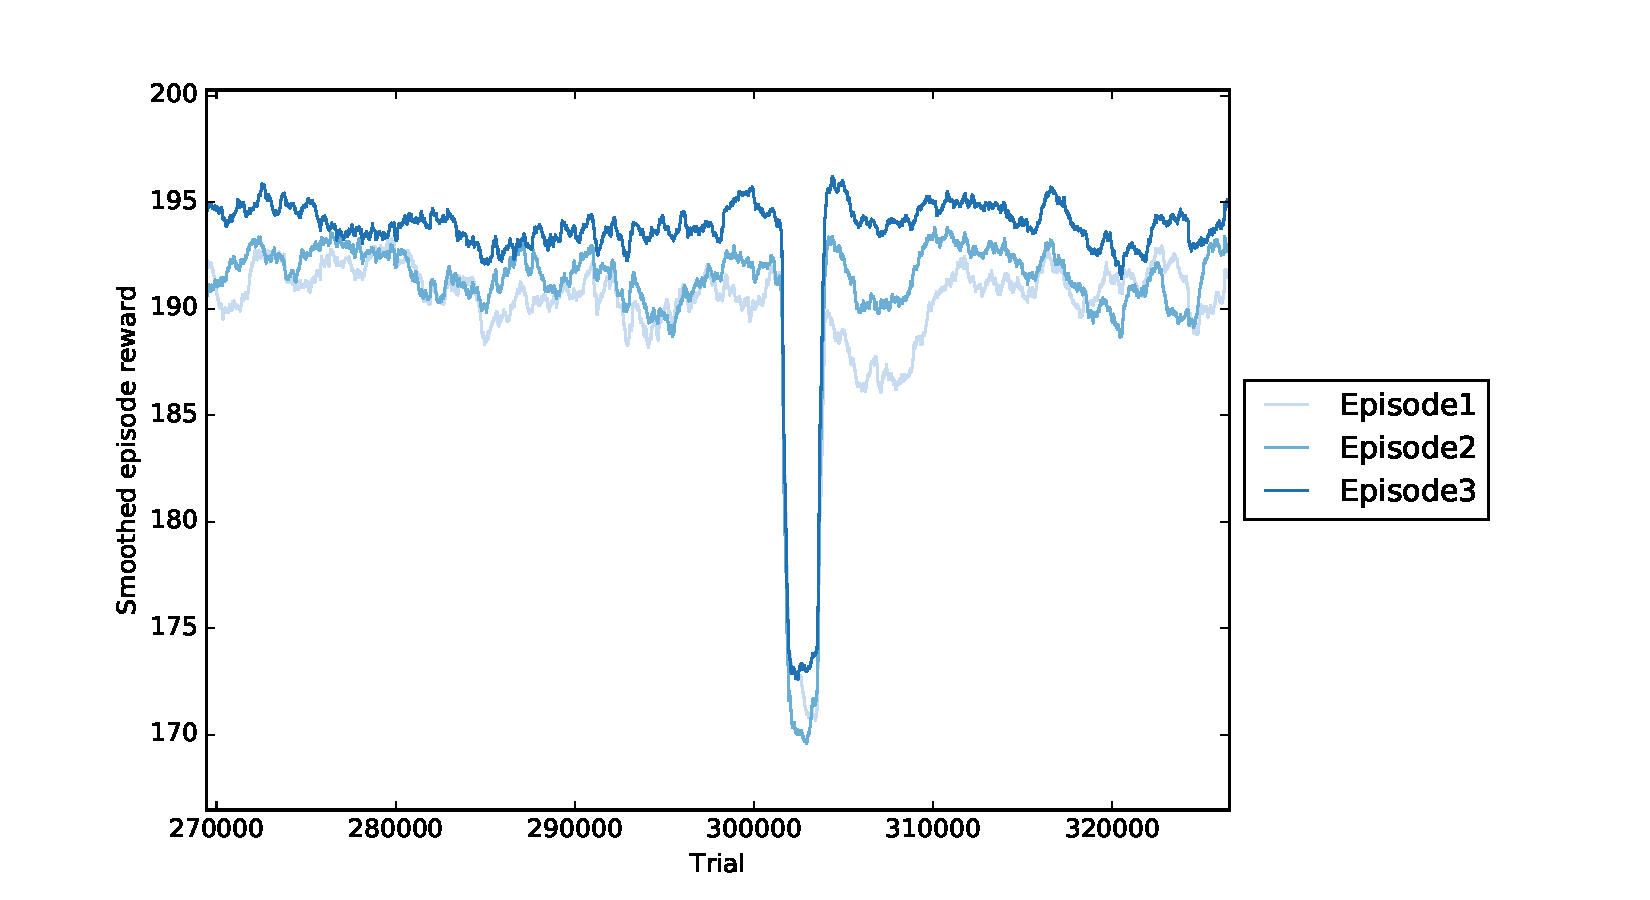
\includegraphics[width=0.8\linewidth]{fig/res_magic_neg10_closeup.pdf}}
	\caption{Episode-wise reward evolution during the training of an
	agent playing trials of 3 episodes with a small negative reward
	at the end of each episode.}
	\label{fig:magic}
\end{figure}

\begin{figure}
	\centering
	\subfloat[][Training permutations]{
		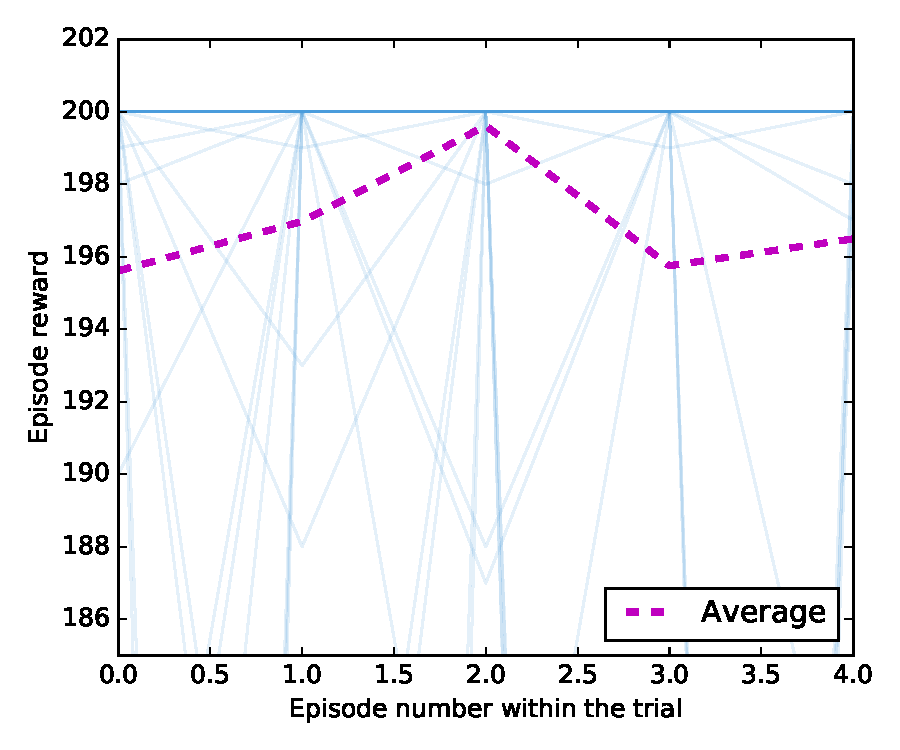
\includegraphics[width=0.45\linewidth]{fig/magic_rewards.pdf}}
	\subfloat[][Testing permutations]{
		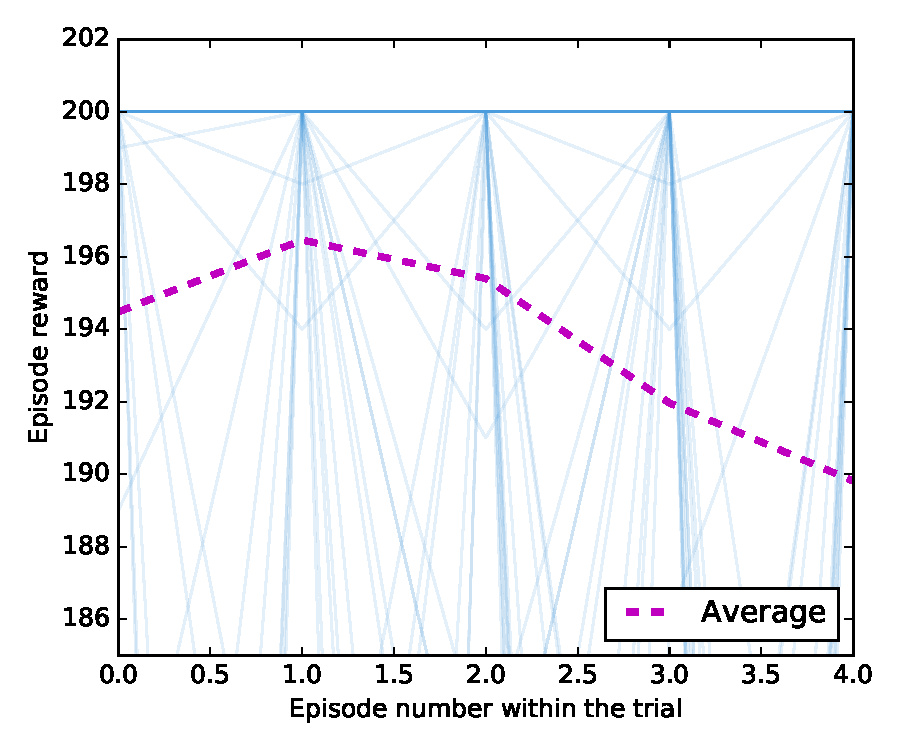
\includegraphics[width=0.45\linewidth]{fig/magic_rewards_unseen.pdf}}
	\caption{Testing performance of the agent trained with the reward
	injection. Several runs are displayed in blue on the same plot, and their
	average is shown as a red dashed line.}
	\label{fig:magic_rewards}
\end{figure}

Even though this is a success, we think there might be a better solution for
problems with a similar reward structure. For example, Wang et al.
\cite{learningtorl} present an experiment (bandits with dependent arms II) 
where the optimal long-term strategy is to start by playing a suboptimal action
voluntarily to gain information that will then allow the agent to play
optimal moves in future episodes. The setting of our experiment doesn't lend
itself to the obligation of abandoning short-term reward for a higher long-term
reward, but adapting it to make room for that type of experiment could be
an interesting lead to follow in future work.\\

We are aware that the results shown so far could seem like they miss one 
of the key promises of meta-learning that were made in the introduction :
the ability to perform tasks that are fundamentally different. Indeed,
one could argue that meta-learning is not really needed in the setting
presented in this chapter as the average reward for the first episode is 
already almost optimal. This is why we propose to test the exact same agent
that was used in the experiments of Figures~\ref{fig:magic} and 
\ref{fig:magic_rewards} for a different CartPole game it has 
actually never been trained to play by inverting one parameter : the reward.
For this experiment, we start giving the agent a reward of +1 at every timestep
only from the moment at which the environment considers it has failed the
episode, until the end of the 200-timesteps episode. 
To our surprise, and perhaps we should emphasize this : 
\textbf{without having been retrained}, the agent learns to fail as quickly
as it can after the first episode. Figure~\ref{fig:magic_magic} shows this
result.

\newpage

\begin{figure}[H]
	\centering
	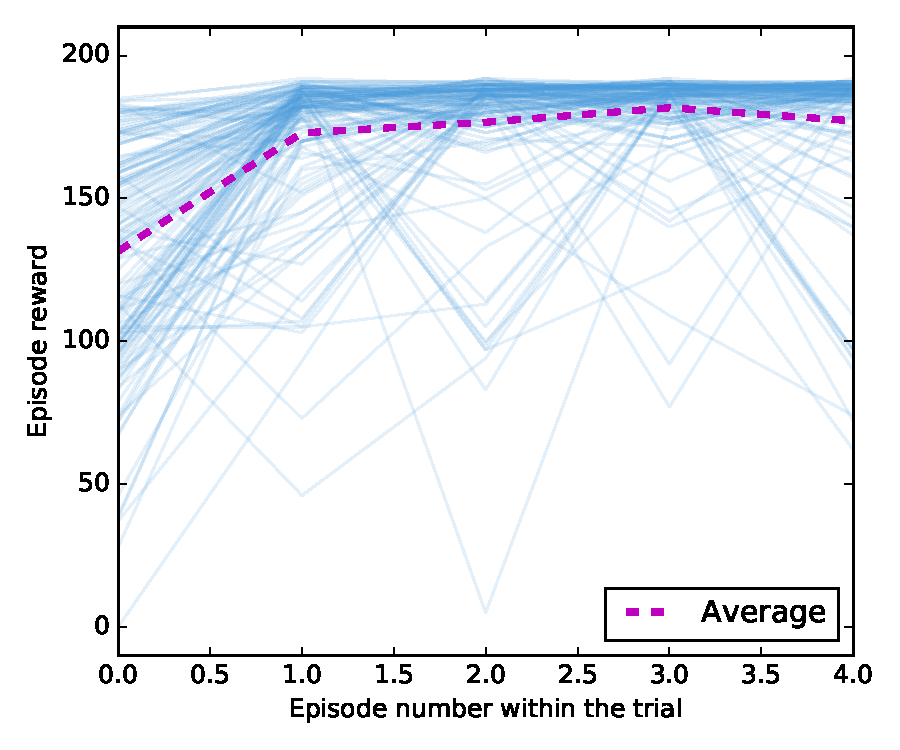
\includegraphics[width=0.8\linewidth]{fig/magic_magic.pdf}
	\caption{Reward per episode for an agent trained to balance the pole,
	tested on a task where a reward is generated as soon as it fails at
	doing what it was trained to do. Each different run is shown in light
	blue; the average of all runs is shown as a dashed red line.}
	\label{fig:magic_magic}
\end{figure}

\subsubsection{Summary}
In this section, we have proposed and successfully tested injecting an
informative process-level negative reward at the end of each episode, 
indicating to the outer algorithm that it should try to keep each episode
running for as long as possible. We trained an agent using this injected
reward on trials of 3 episodes and found that it performed well on each
episode, but that performance generally increased between episodes.\\

We also tested this agent on a completely new problem, where it was implicitly
asked to fail at what it had been trained for as quick as possible. The results
showed that the agent quickly learned to fail after the first episode, increasing
dramatically its average reward over following episodes.







\chapter{Conclusions}
\begin{quotation}
\noindent ``\emph{By far the greatest danger of artificial intelligence
	is that people conclude too early that they understand it.}''
\begin{flushright}\textbf{Eliezer Yudkowsky}\end{flushright}
\end{quotation}
\vspace*{0.5cm}

After having reviewed the foundations of artificial neural networks and
reinforcement learning, we went through the reasons why meta-learning is
interesting and useful: not only it allows one to avoid choosing, designing
or parametrising complex task-related strategies to accelerate training, but
most importantly, it allows for agents to learn highly efficiently problems
that have the same structure and to generalise over the parameters of the 
structure -- bluntly put, one can reuse an agent without retraining it, as long
as the problem is similar and the meta-learning agent has seen enough
variation in the training distribution.\\

We have reproduced one experiment originally setup by Wang et al. 
\cite{learningtorl} and Duan et al. \cite{fastrlviaslowrl} which consisted
in meta-learning dependent 2-armed bandit problems. While we achieved the
same results as the two seminal papers cited above, we extended the results
discussion to the dynamics of meta-learning such a problem, showing how
the meta-learning agent develops its strategy to learn a bandit problem faster
and faster. We also studied its generalisation capability for the whole
range of parameters of this problem.\\

Meta-learning was extended to a new set of experiments based on the CartPole
environment. We designed a distribution of CartPole problems by shuffling
the state observation received by the agent (without informing the agent
of the mapping between values and their meaning), and by permutating 
the agent's actions randomly at the start of training trials.\\

We have shown that even though, surprisingly, the agent was able to learn
to discover which problem it was playing in one episode, meaning that:
\begin{enumerate}
	\item it was able to make sense of an unordered set of values in input;
	\item it was able to learn the consequences of its actions;
	\item it could perform 1) and 2) in time to be able to balance the
		pole for a long enough time to succeed the episode.
\end{enumerate}
Although the performance of the agent was near optimal, we found that letting
the agent play for at least two episodes increased its performance as it
was able to learn about the environment and take consequential action in
later episodes to improve its success rate. Quite surprisingly also,
the meta-learning agent performed better in environments which were more
difficult, and the difference between single-episode and multi-episode trials
increased as the problems grew harder and both were tested on previously unseen
problems.\\

There are still parameters to choose manually when designing a meta-learning
agent, and their tuning provides for some interesting dynamics in the 
performance of a trained agent. We have studied how the discount factor
and the number of episodes per trial
played an important role in the evolution of episode-wise reward during the 
training of a meta-learning agent.
We have also tried to understand how a meta-learning agent handled playing
more episodes than what it had been trained for.\\

This deep look into the workings of our agent and its reaction to different
hyperparameters helped us understand an inherent flaw in the reward structure
of the CartPole problem forbidding the agent to perform at its best for
as many episodes as possible, as soon as it could. Indeed, a continuous
stream of rewards of +1 at each timestep drowned the information of "lost
episodes" to the meta-learning agent.\\

This discovery led us to propose a simple way to inject an informative reward
at the end of each episode to allow the agent to play at its best performance
as soon as it could, learning and passing information on to following episodes
so that they could in turn perform even better. After having successfully
trained an agent to balance the pole in CartPole with this informative reward,
we tested it on the novel, unseen task of failing at what it had been trained
to do by starting to give it positive reward only after its failure. To
our surprise, the agent managed to learn to fail within the first episode
of its trials, later taking action to fail its episodes as quickly as it 
could. This new problem was sucessfully learned only within \textbf{one} episode
without having to be retrained.\\

\section{Future work}
There is still much to explore in meta-learning. For instance, could a 
meta-learning agent learn to play problems generated from different environment?
What would be the similarity constraints for it to work? If the agent does
manage to learn to perform well in different environments, could it then
learn to play in a totally unseen environment? Once again, in that case,
what would be the requirements in terms of similarity to ensure success?\\

Furthermore, could environments with fundamental differences (different 
dimensionalities of the state and action sets) be learned by the same agent?\\

We are very confident in the multi-tasking capabilities of the meta-learning
agent, and its ability to add an interpretation level between itself and the 
state, both input-wise (when it receives observations) and output-wise (when
it performs actions); and hope that there will be a strong interest in 
researching the limits of its performance.\\

We suspect that adapting the architecture presented by Wang et al. to allow
the outer algorithm to access more information that is implicitly or
explicitly available to strategy designers (e.g. have knowledge of total 
episode rewards instead of timestep-only rewards) could lead to an overall 
better learning algorithm.\\


\section{Source code}
The source code for our agent, and also the code used to run all the
experiments of this work has written in Python 3 \cite{python3} using
Tensorflow \cite{tensorflow}. It is available at the following url:
\url{https://github.com/fhennecker/meta-reinforcement-learning}.


%------------------------------------------------------------------------------
% Appendix

% \appendix
% \chapter{First appendix}

\backmatter
% \printindex % use makeindex
\bibliographystyle{plain}
\bibliography{biblio} 

\end{document}


